\chapter{Results}
\section{EEG results}
In this thesis, the EEG results will be presented in a descriptive manner, in which we describe the outcomes presented in the obtained oscillatory waveforms (Figures \ref{fig: Waveforms control: occipital}, \ref{fig: Waveforms stroke: occipital}) and topographies (Figure \ref{fig: 3D topographies control group}, \ref{fig: 3D topographies stroke group}). Further, statistical analyses will be conducted in the future.  \\
As expected from our previous study conducted by Matamala-Gomez et al. (in preparation), in our research we also observed a greater synchronization effect in rhythmic sequences compared to random sequences in all three ROIs (occipital, temporal, and sensorimotor) and in each experimental block (auditory, visual, and audiovisual). Moreover, as in the previous study, we also observed a synchronization effect in the sensorimotor cortex when presenting auditory and audiovisual sensory inputs in rhythmic sequences at 2 Hz, in both healthy population and patients with stroke (Figures \ref{fig: Waveforms stroke: occipital}, \ref{fig: Waveforms stroke: temporal}, \ref{fig: Waveforms stroke: sensorimotor}). However, visually, the topographies tend to show that mean power spectrum activity is lower in patients with stroke compared to healthy subjects.\\
This tendency should be confirmed using proper statistical analysis. From the topographical representation of these effects (see Figures \ref{fig: 3D topographies control group} and \ref{fig: 3D topographies stroke group}), we can see clear differences in the sensorimotor effects in the stroke patients compared to the control group. For example, in the Affected hemisphere in stroke patients (left-hemisphere view), the activation observed in the sensorimotor cortex in the patients is more lateral and posterior, showing less magnitude. Also in the audiovisual condition, the activation in the healthy hemisphere is less and being more anterior compared to the control group. \\
For the visual sensory input, in our study we also observed a higher synchronization of the visual input within the occipital cortex in rhythmic sequences, but not showing entrainment at the sensorimotor cortex. This result was also observed in the previous investigation from Matamala-Gomez et al. \\
Overall the present new results tend to show clear brain reorganization effects in the sensorimotor cortex, showing less entrainment and variability in these regions, probably due to the presence of a lesion in the motor system.  
\begin{figure}[htbp]
    \centering
    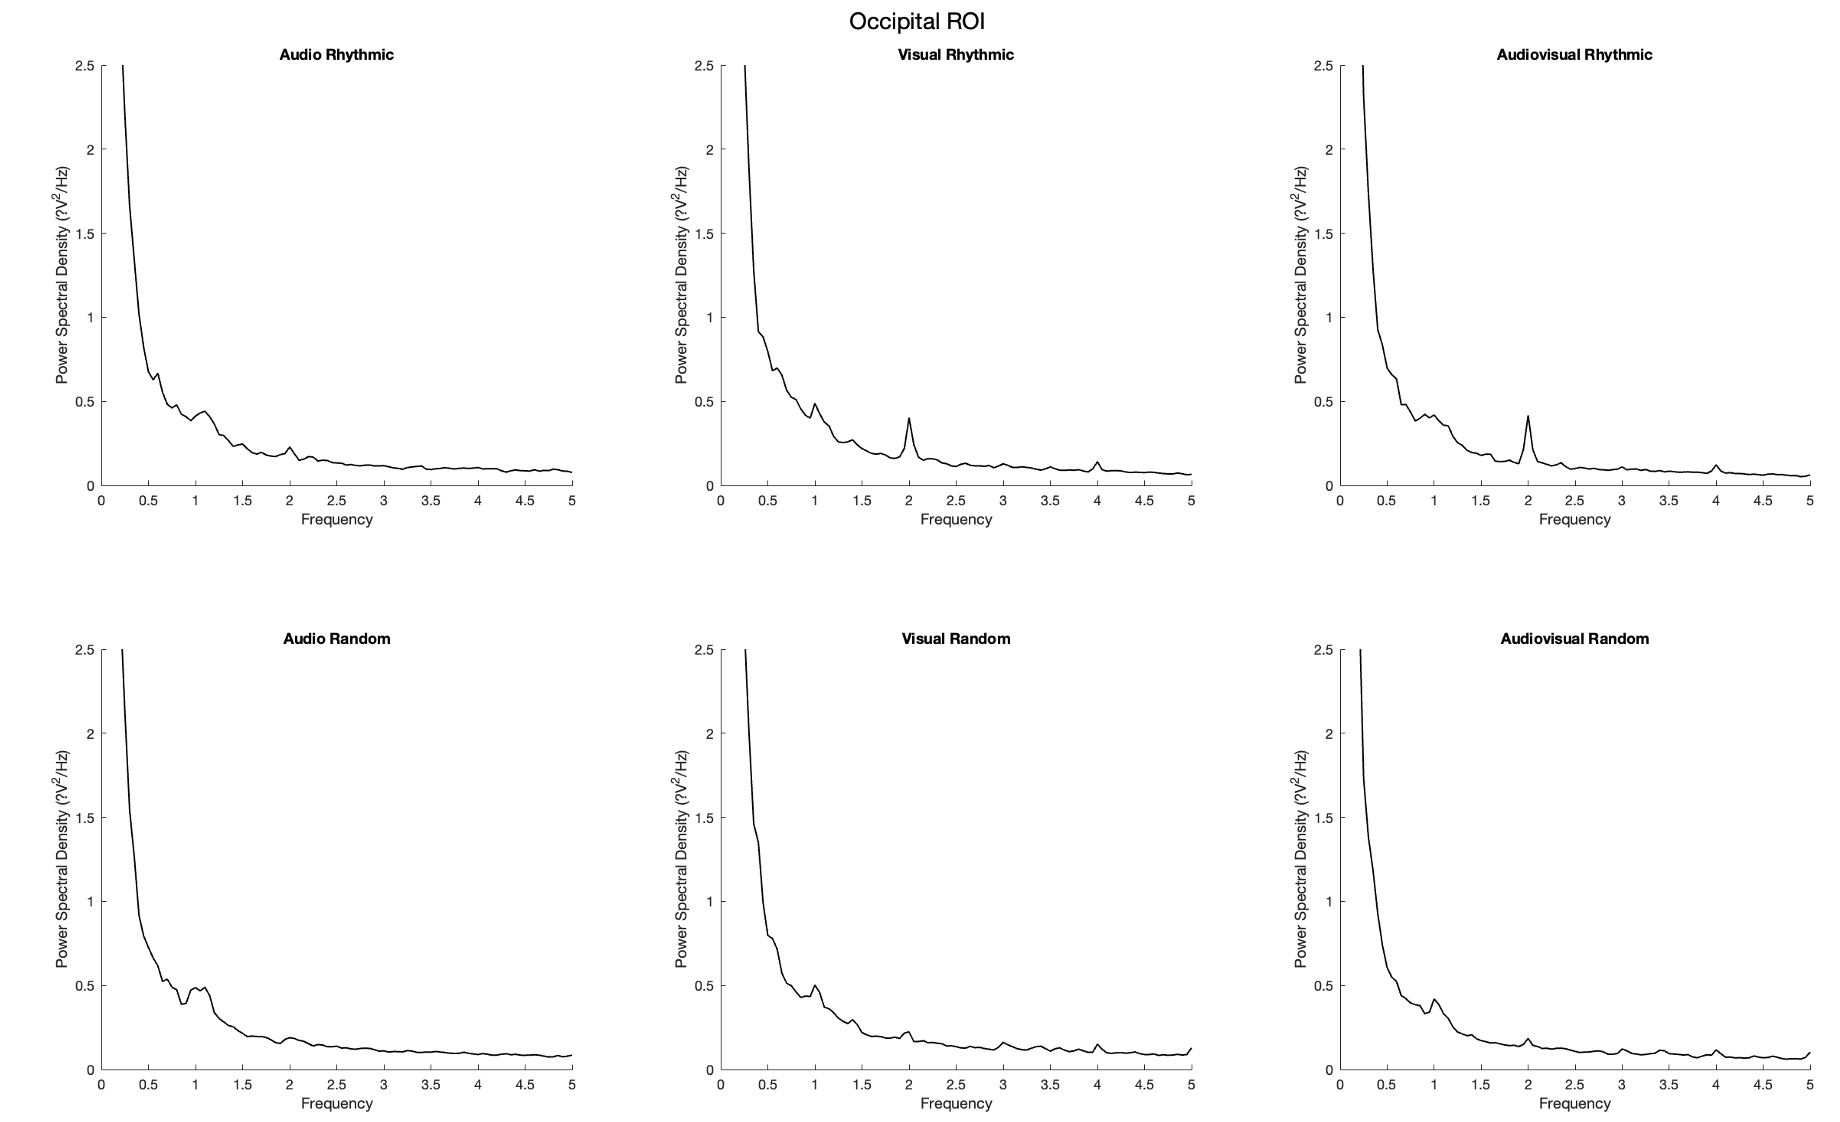
\includegraphics[width=0.75\textwidth]{healthy_images/occipitalROI_graph.png}
        \caption{Power spectrum of the Occipital ROI: control group}
        \label{fig: Waveforms control: occipital} 
\end{figure}
\begin{figure}[htbp]
    \centering
        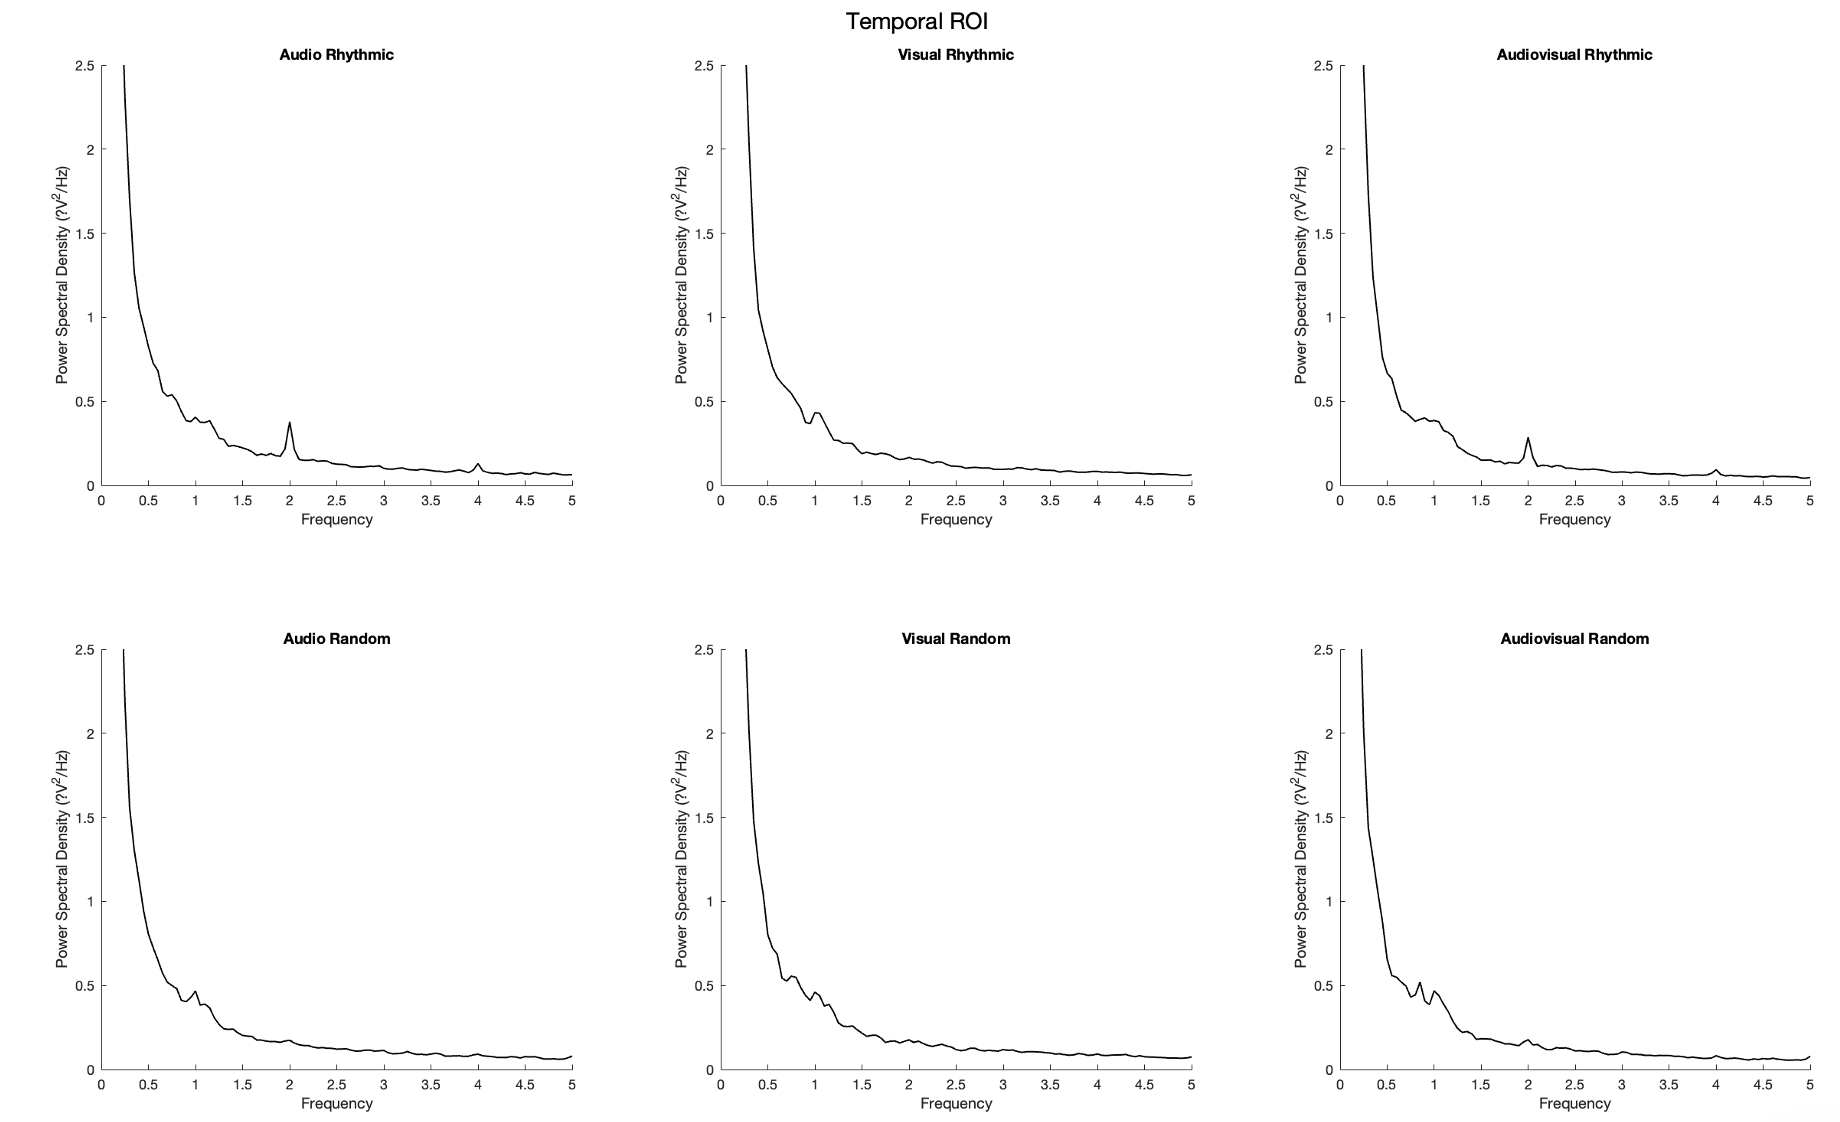
\includegraphics[width=0.75\textwidth]{healthy_images/temporalROI_graph.png}
        \caption{Power spectrum of the Temporal ROI: control group}
        \label{fig: Waveforms control: temporal}   
\end{figure}
\begin{figure}[htbp]
    \centering
    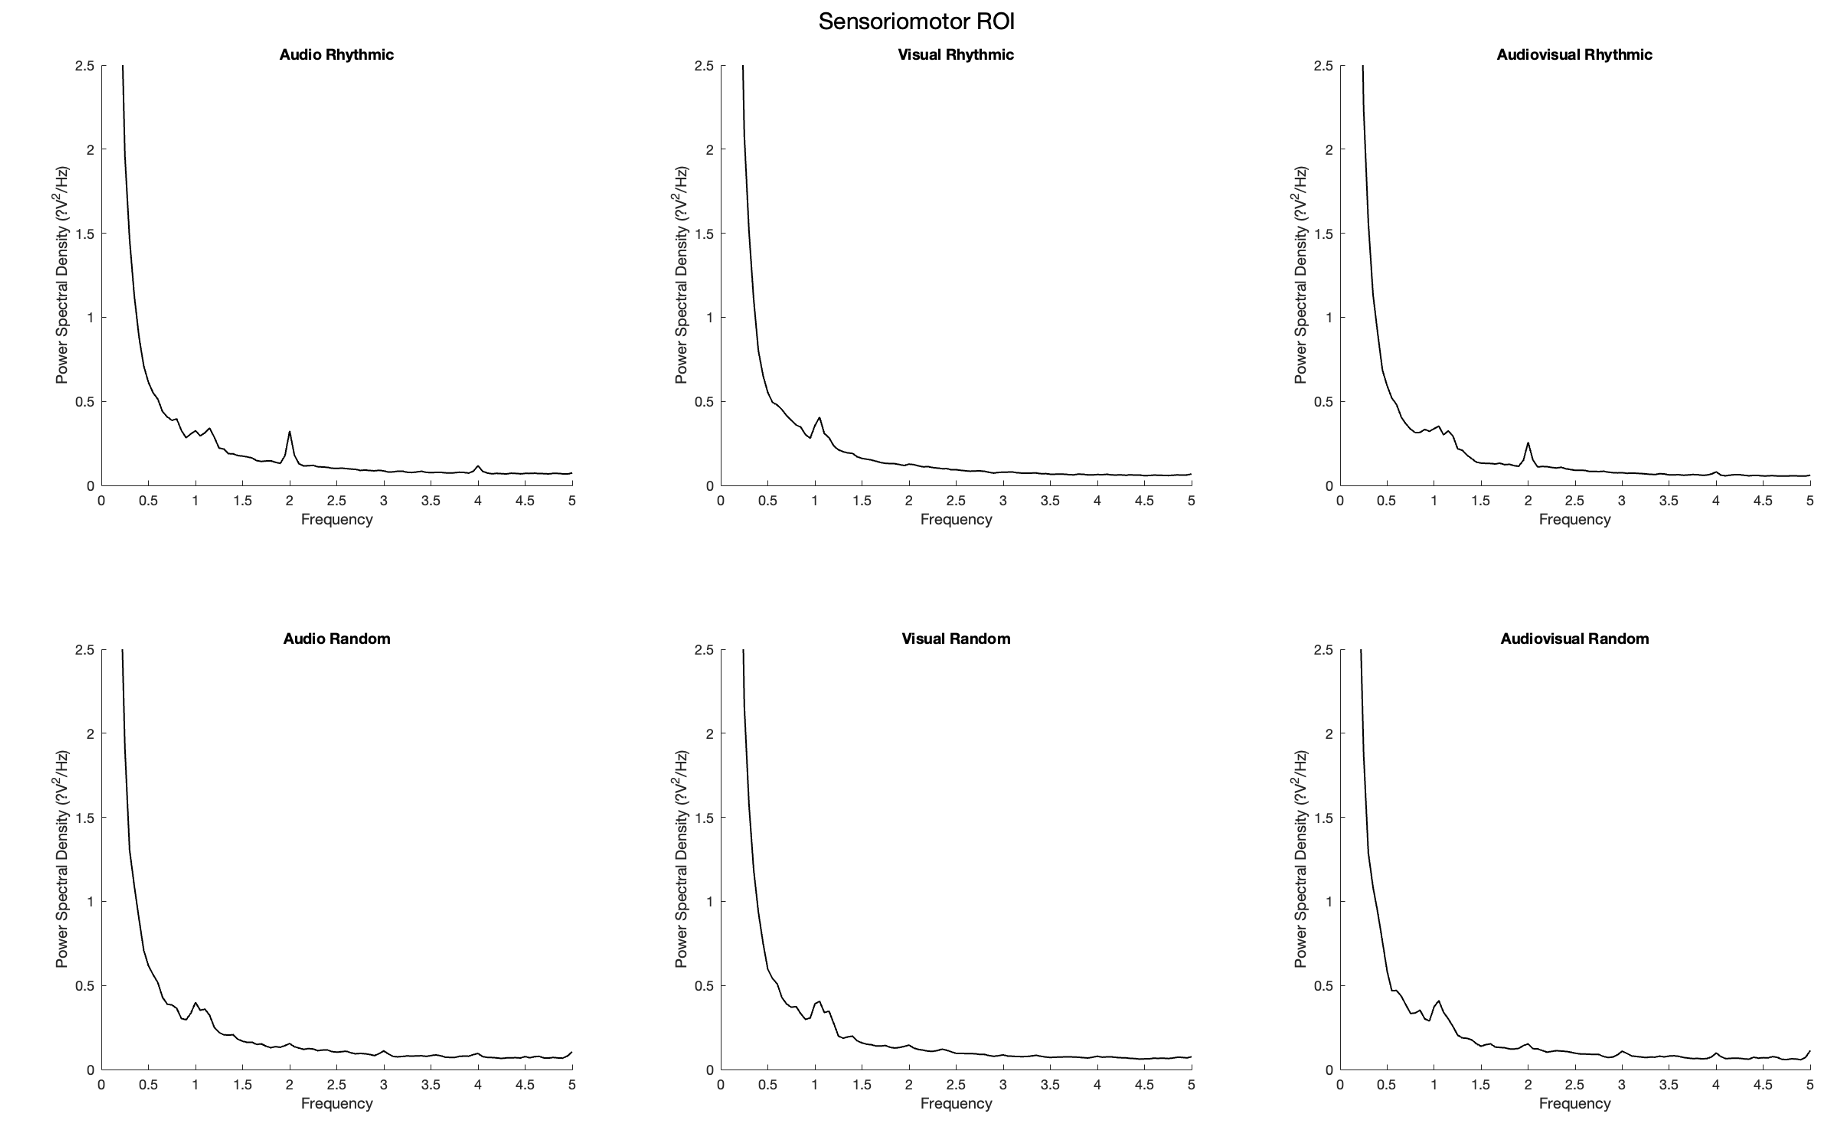
\includegraphics[width=0.75\textwidth]{healthy_images/sensorimotorROI_graph.png}
    \caption{Power spectrum of the Sensorimotor ROI: control group}
    \label{fig: Waveforms control: sensorimotor}   
\end{figure}

\begin{figure}[htbp]
    \centering
    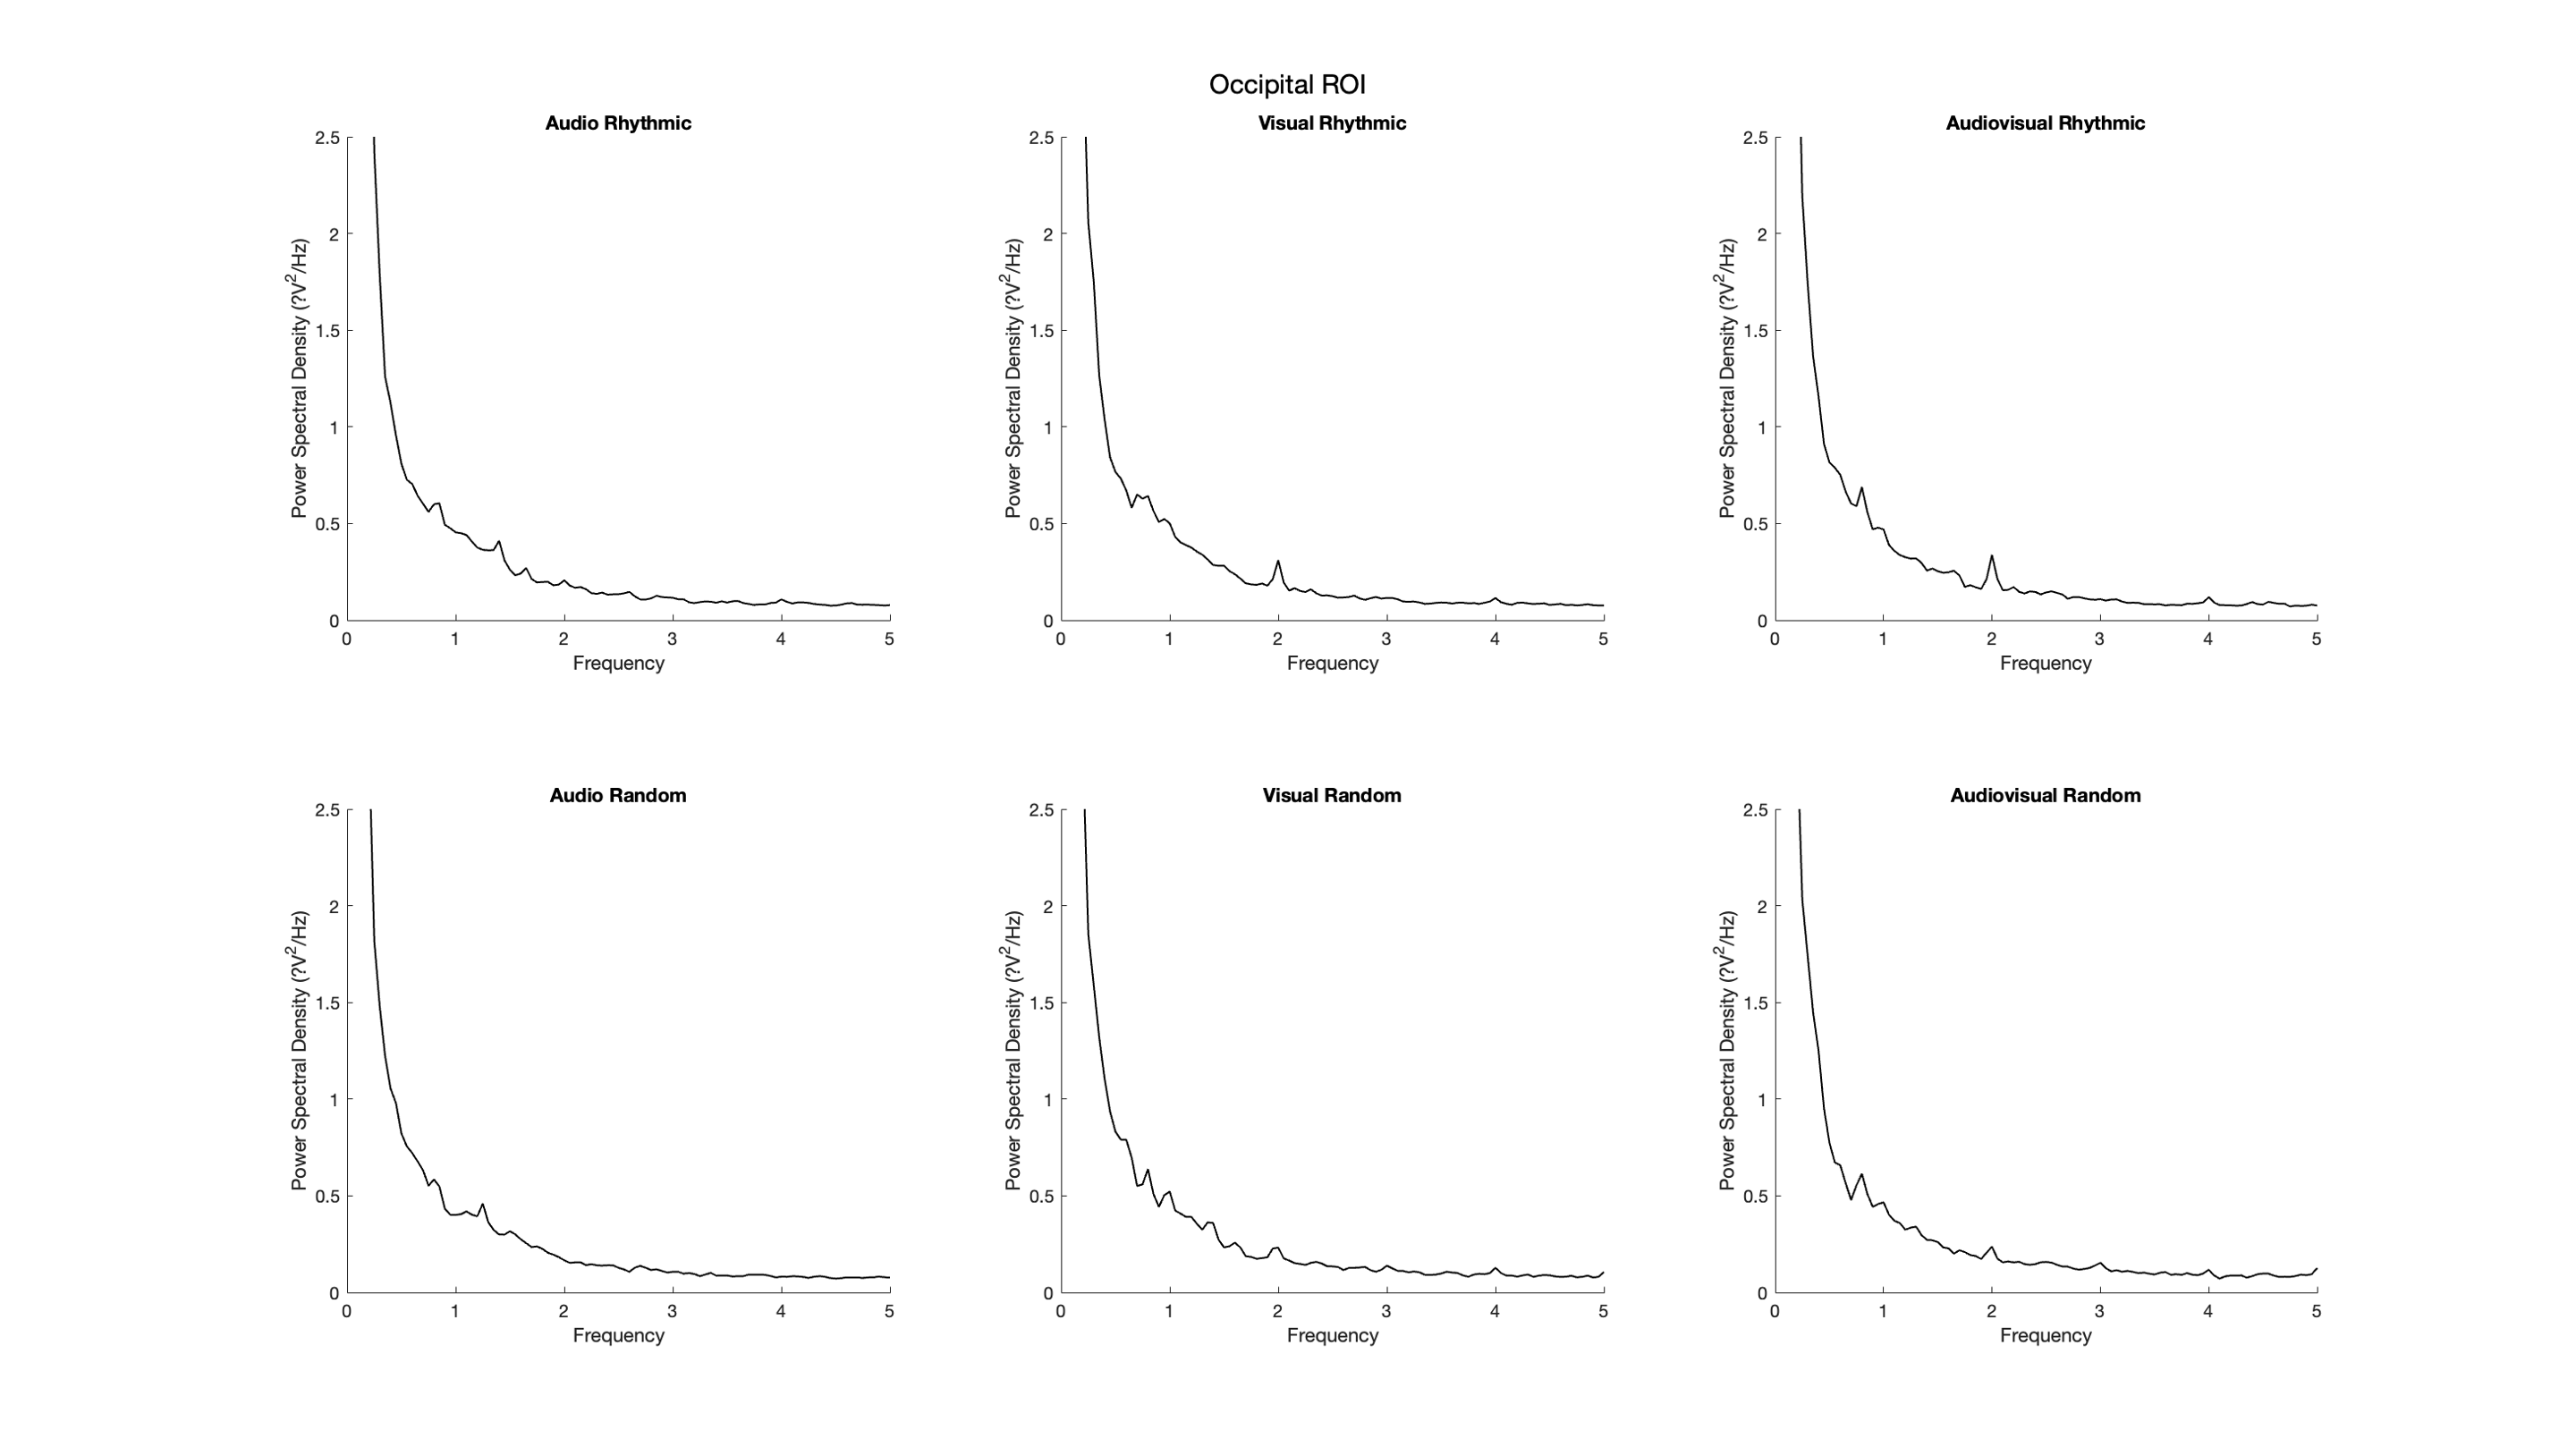
\includegraphics[width=0.9\textwidth]{stroke_images/occipital_roi.png}
    \caption{Power spectrum of the Occipital ROI: stroke group}
    \label{fig: Waveforms stroke: occipital} 
\end{figure}  
\begin{figure}[htbp]
    \centering
    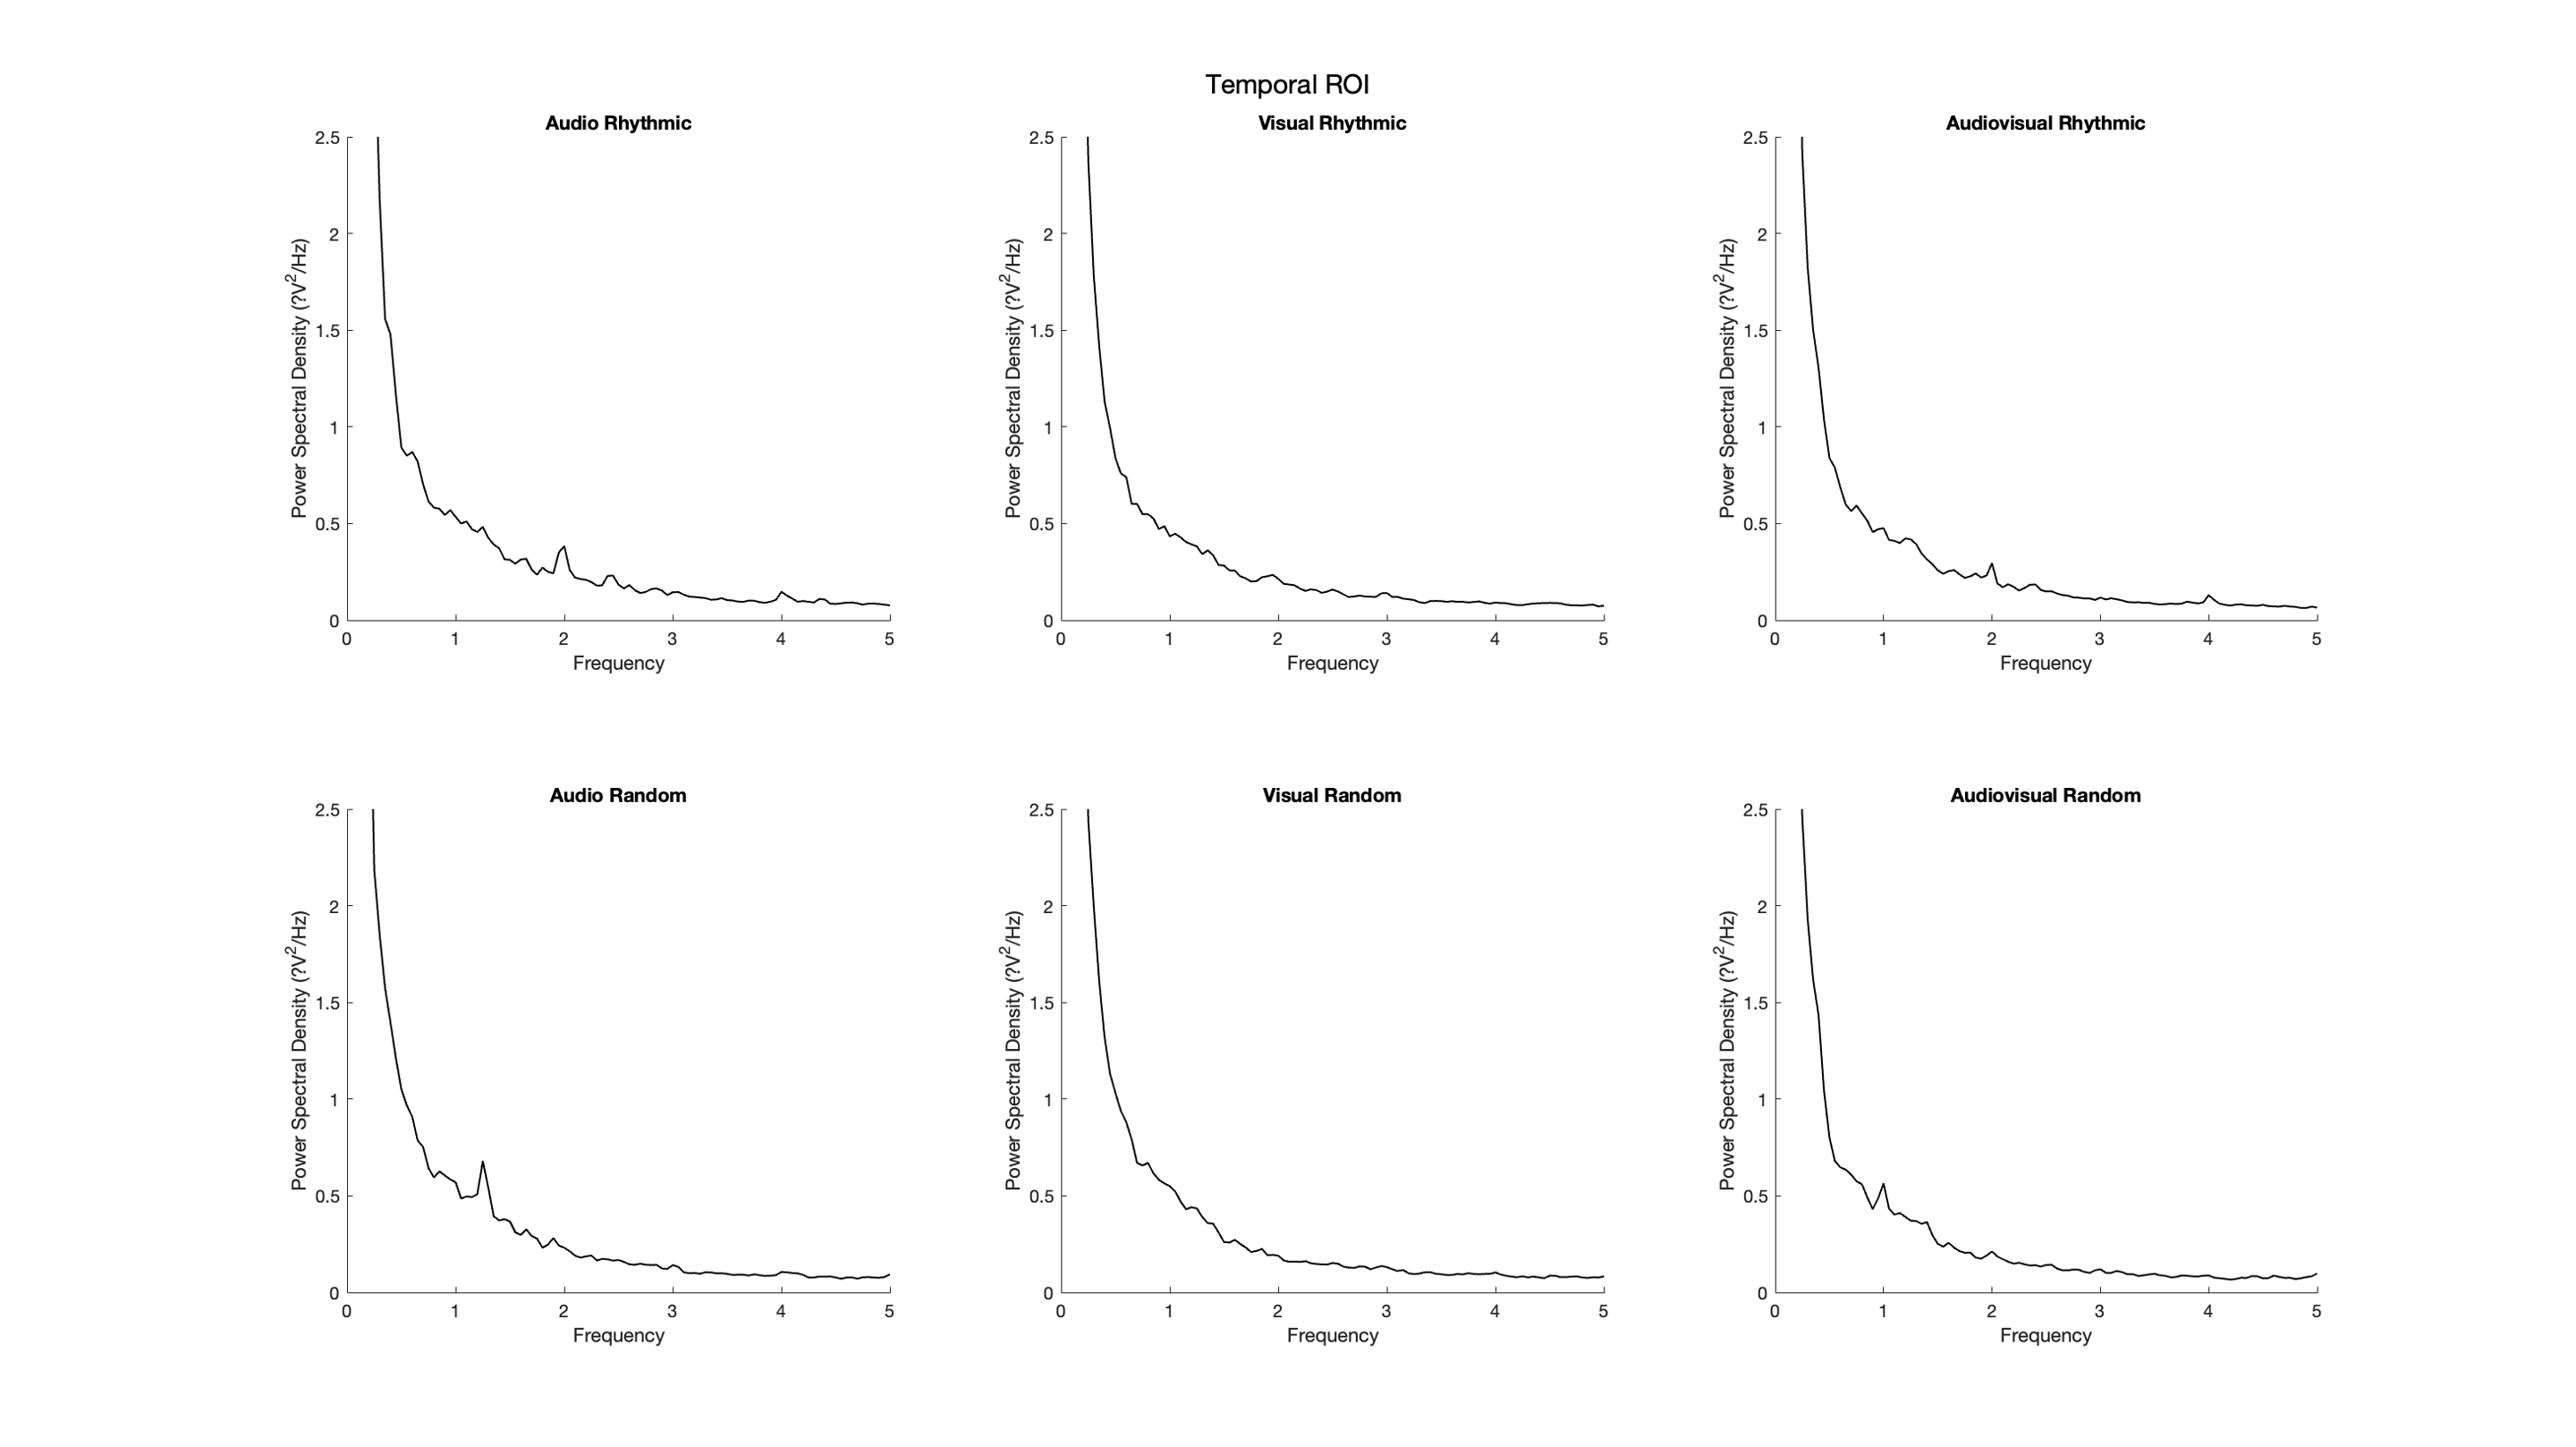
\includegraphics[width=0.9\textwidth]{stroke_images/temporal_roi.png}
    \caption{Power spectrum of the Temporal ROI: stroke group}
    \label{fig: Waveforms stroke: temporal}   
\end{figure}
\begin{figure}[htbp]
    \centering
    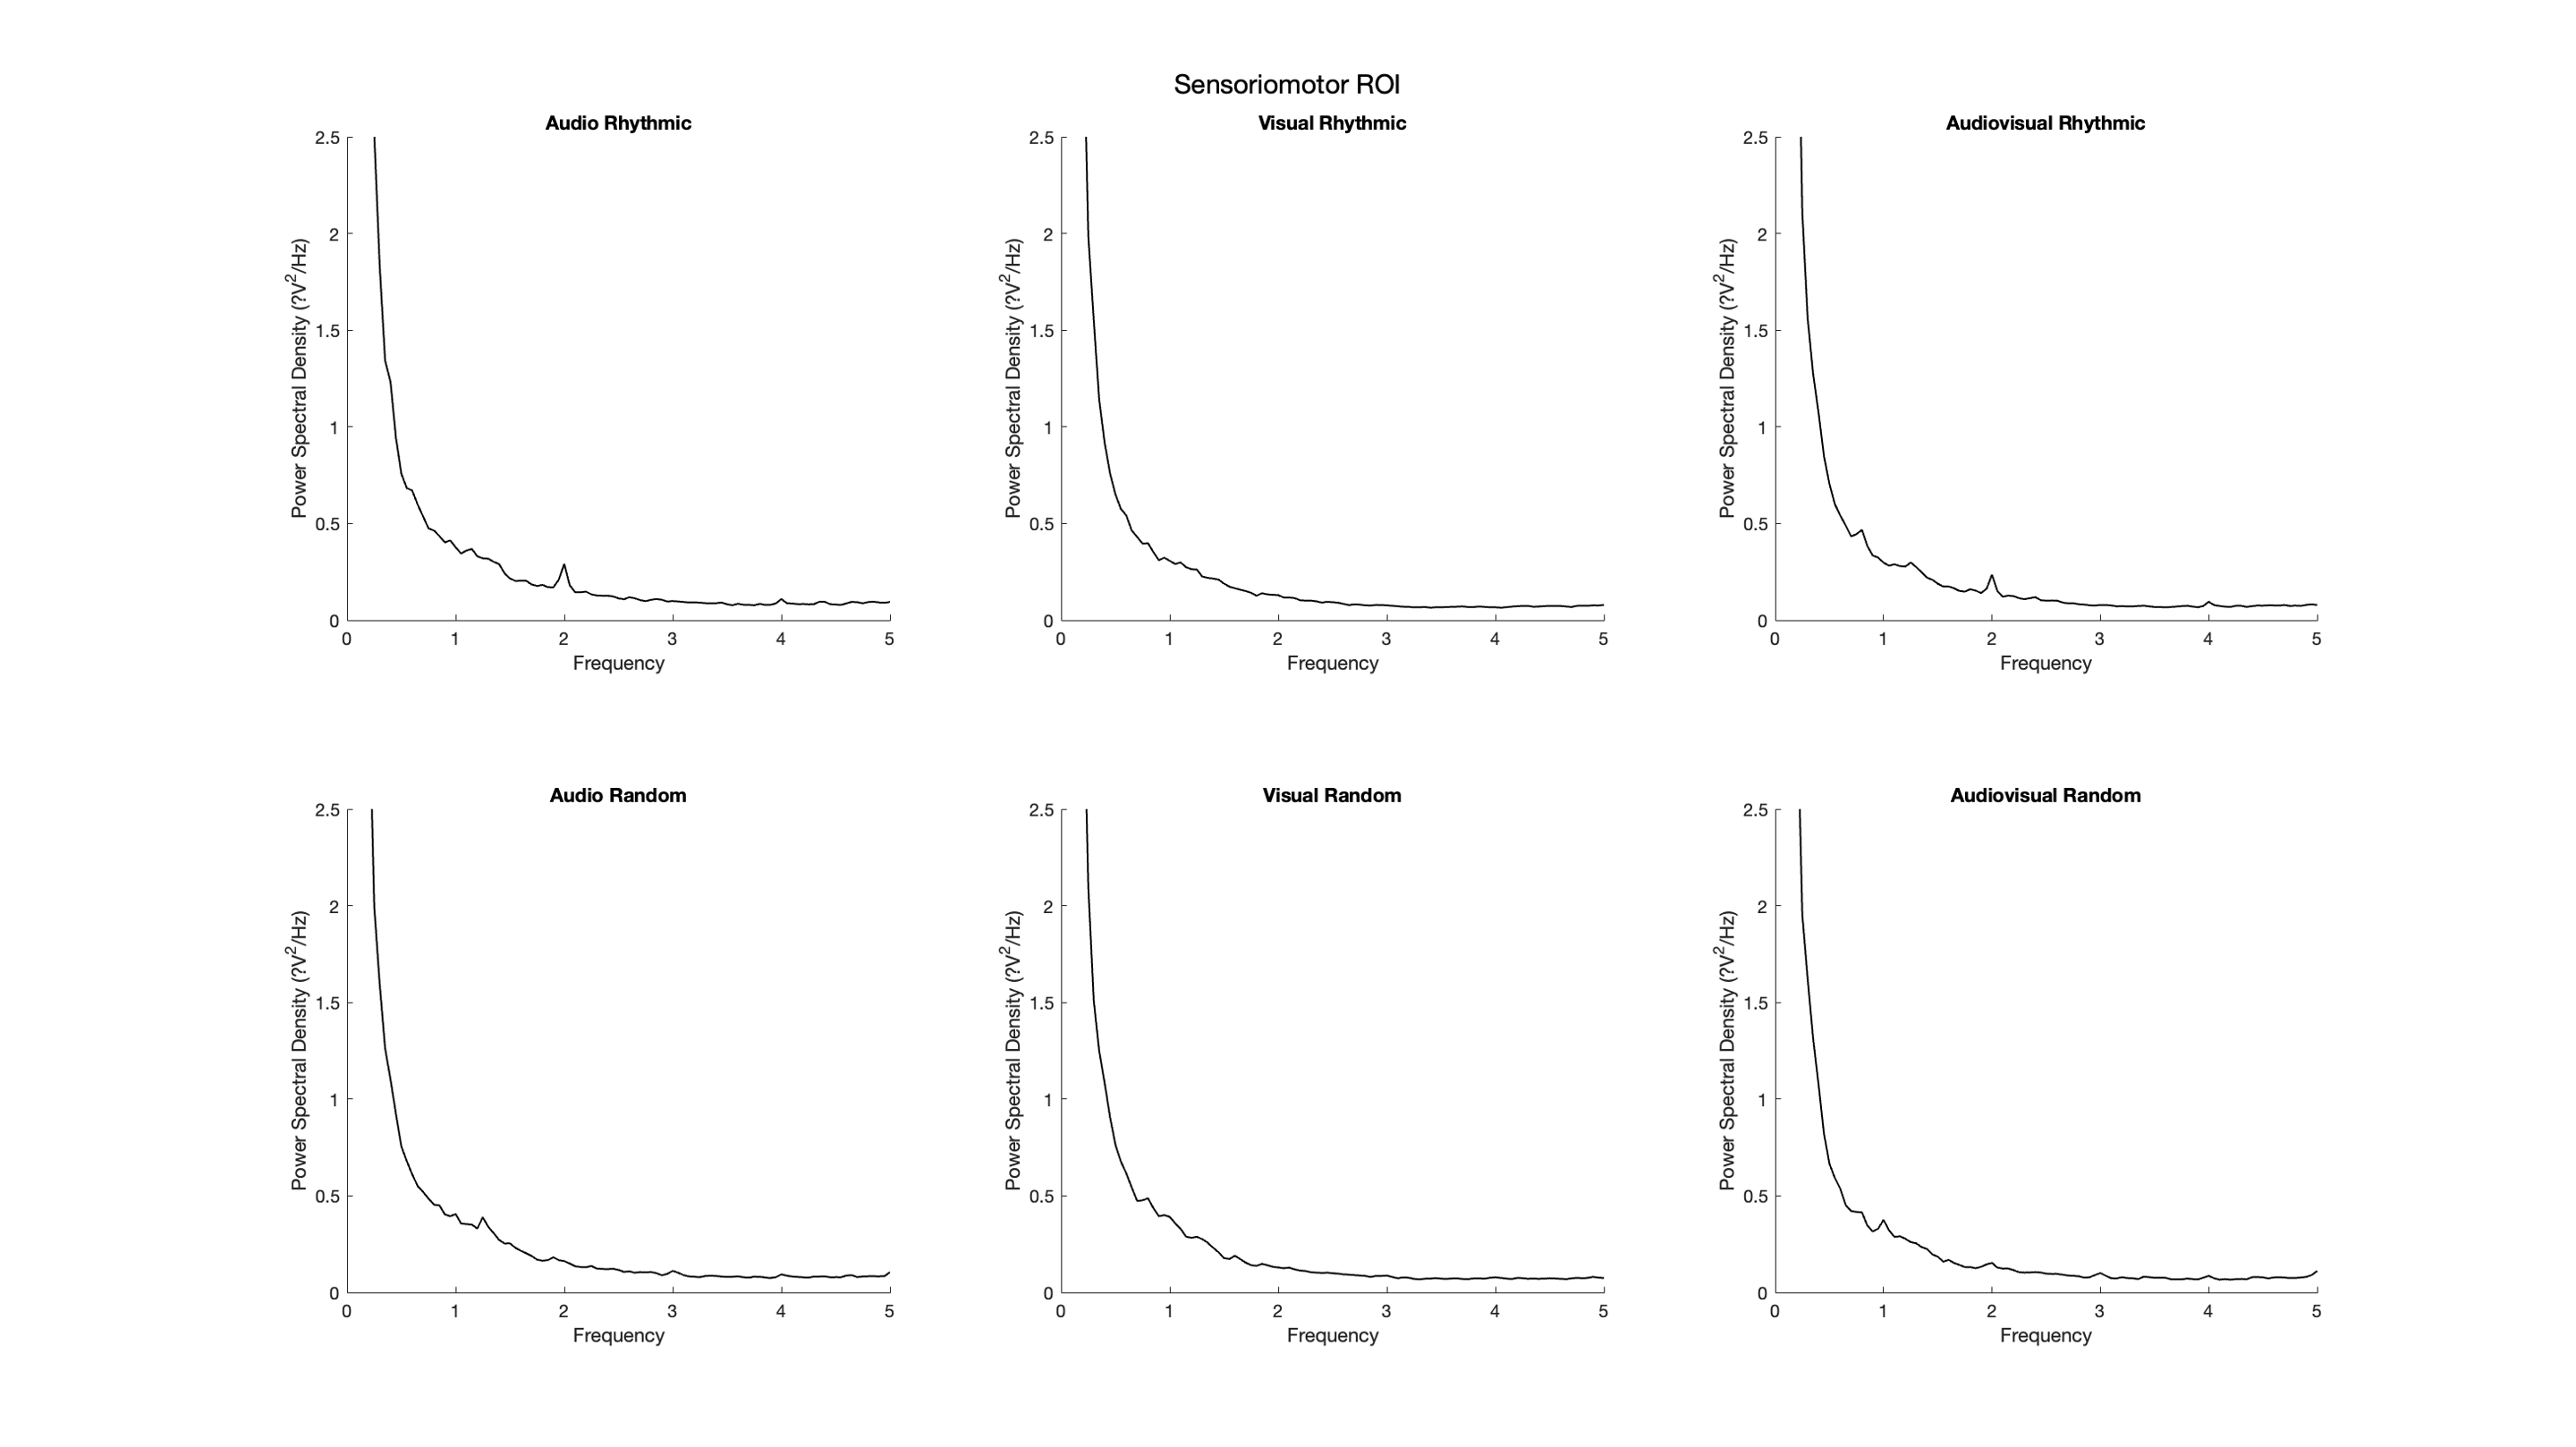
\includegraphics[width= 0.9\textwidth]{stroke_images/sensorimotor_roi.png}
    \caption{Power spectrum of the Sensorimotor ROI: stroke group}
    \label{fig: Waveforms stroke: sensorimotor}   
\end{figure}

\begin{figure}[htbp]
        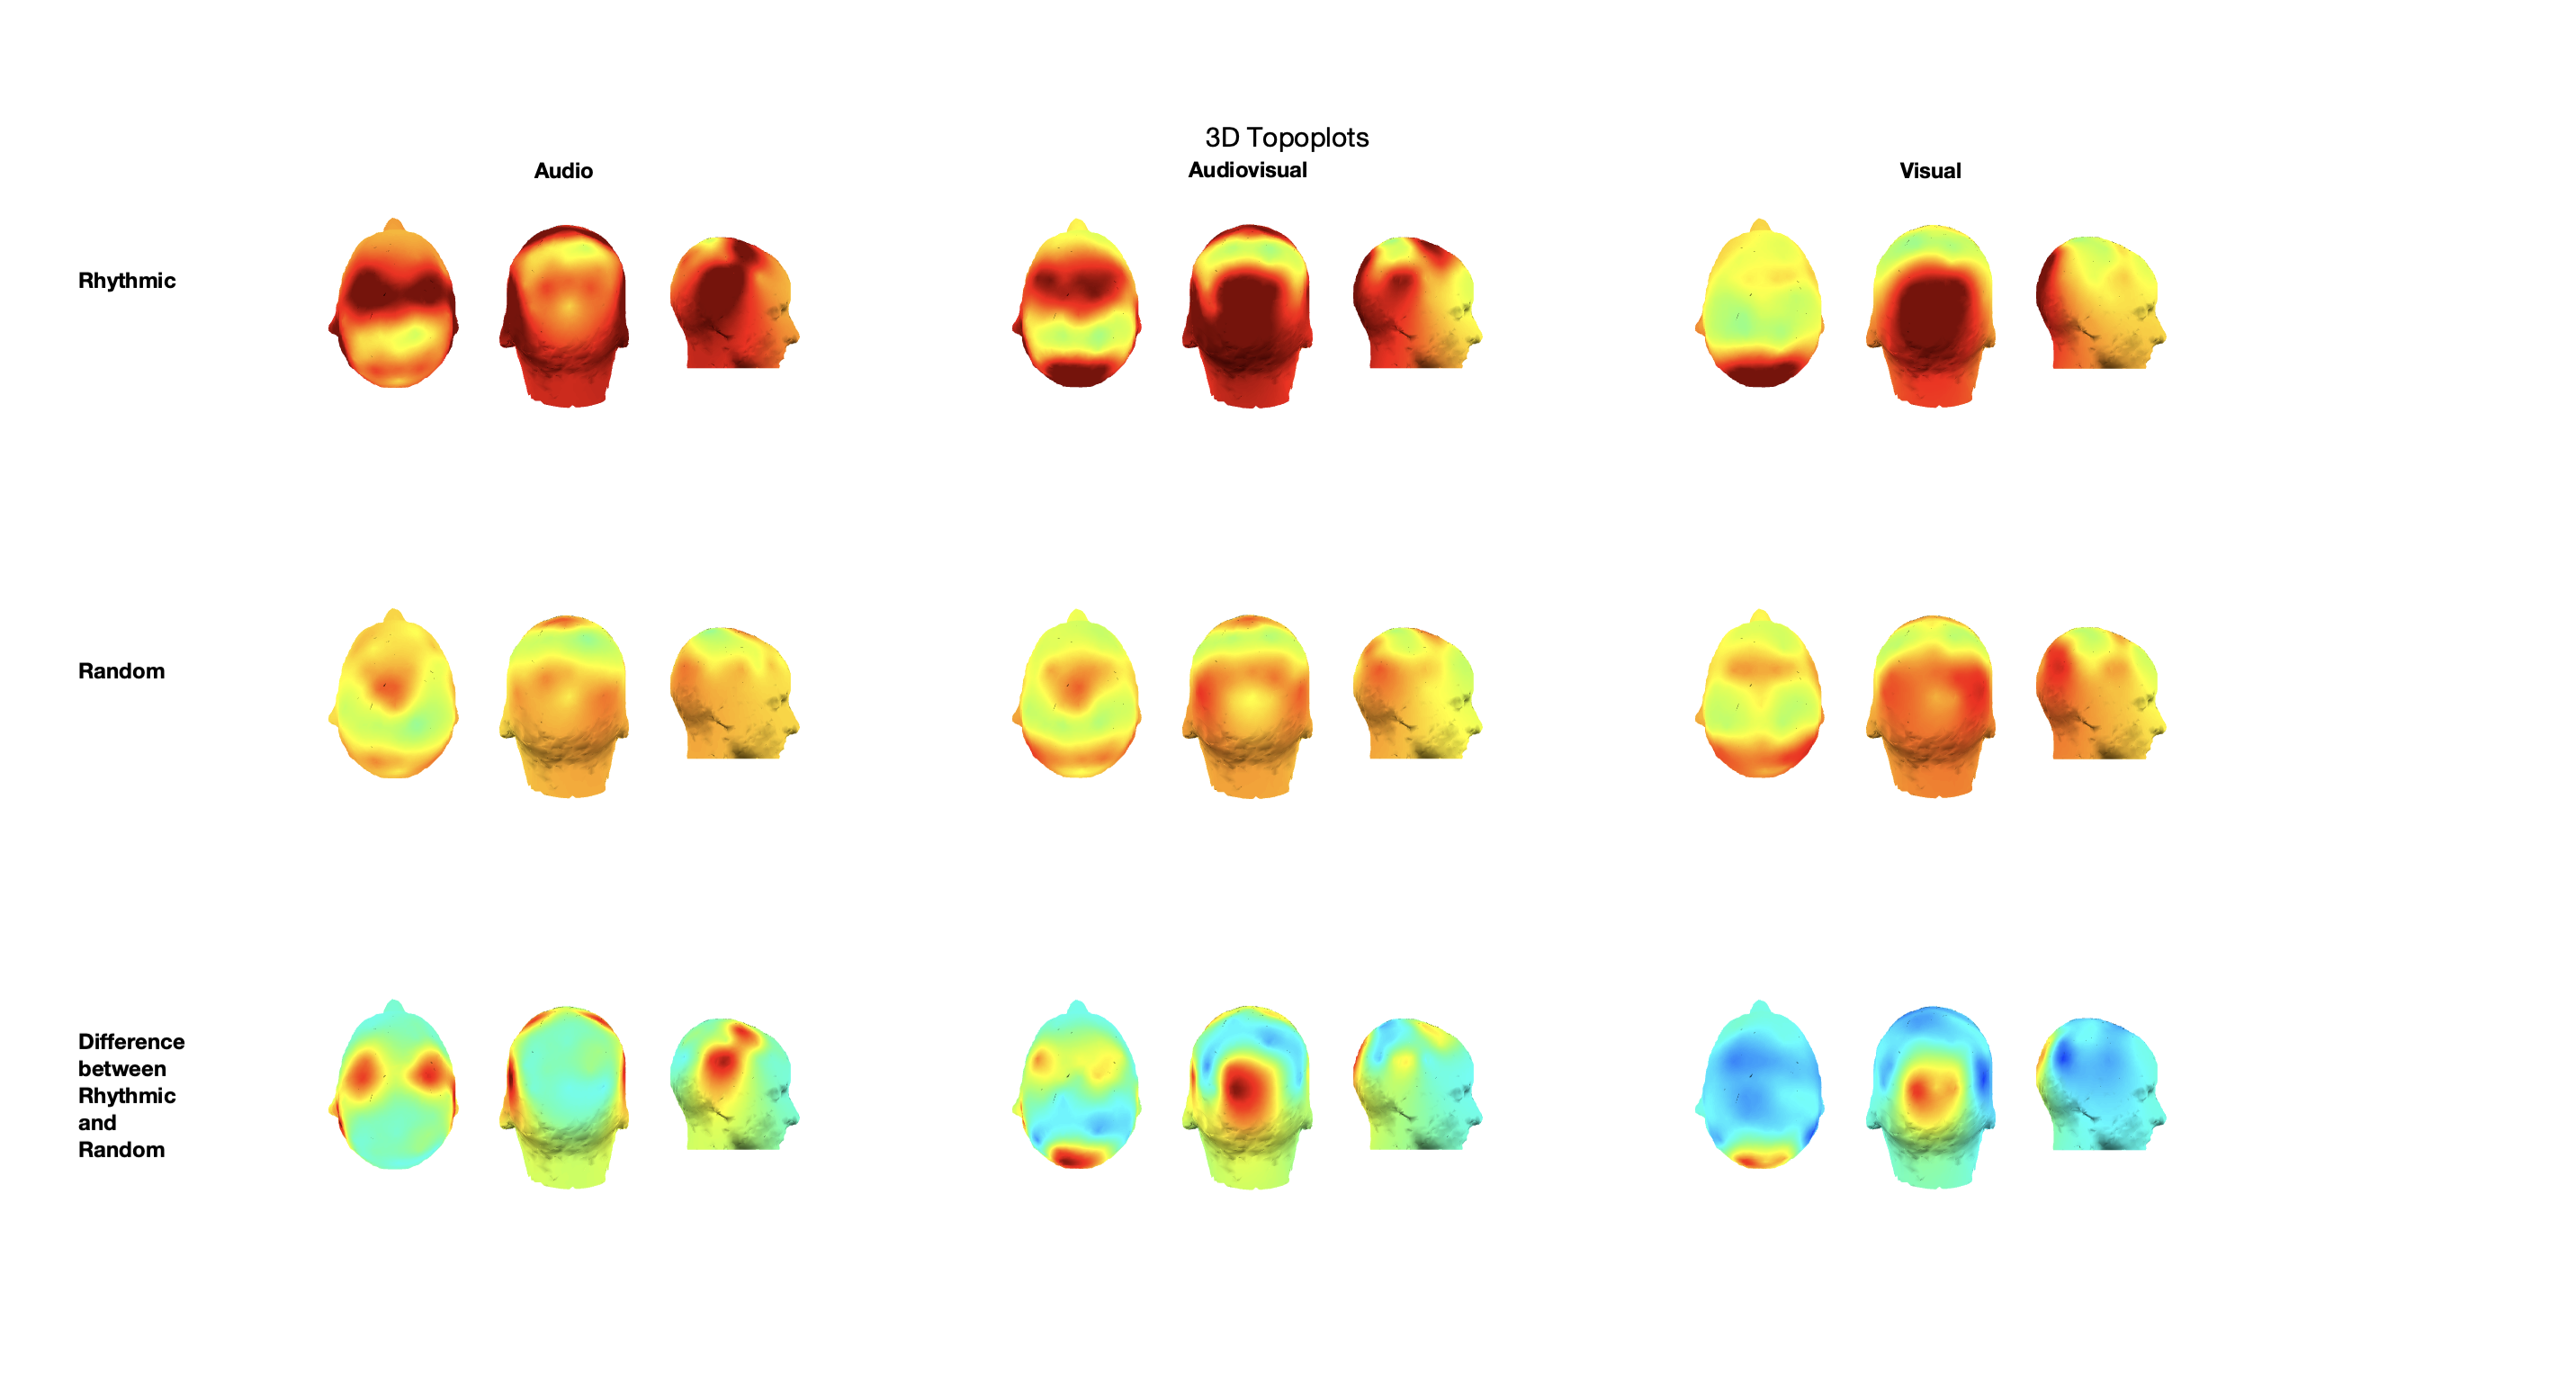
\includegraphics[width=1\textwidth]{healthy_images/3d_topo.png}
        \caption{3D topographies related to the activity in the control group}
        \label{fig: 3D topographies control group} 
\end{figure}
\begin{figure}
    \includegraphics[width=1\textwidth]{stroke_images/3d_topographies.png}
        \caption{3D topographies related to the activity in stroke population}
        \label{fig: 3D topographies stroke group}   
\end{figure}

\clearpage
\section{Subjective report questions results}
In the subjective report questions results, we calculated the mean difference between the values obtained from the subjective questions provided after the presentation of each sensory inputs in each experimental block (auditory, visual, audiovisual). We compared the mean difference between rhythmic and random sequences for the experimental (stroke patients) and control group (healthy subjects). \\
The results show a significant mean difference between the sensory inputs presented in the rhythmic and random sequences in both groups (healthy and patients with stroke), and in all three experimental blocks (auditory, visual, and audiovisual), presenting higher values in rhythmic compared to random sequences in both healthy and patients with stroke group (see \textit{p} values reported in Figure \ref{fig: significance rhythmic-random}).
\begin{figure}[htbp]
    \centering
    \begin{subfigure}[htbp]{0.33\textwidth}
        \centering
        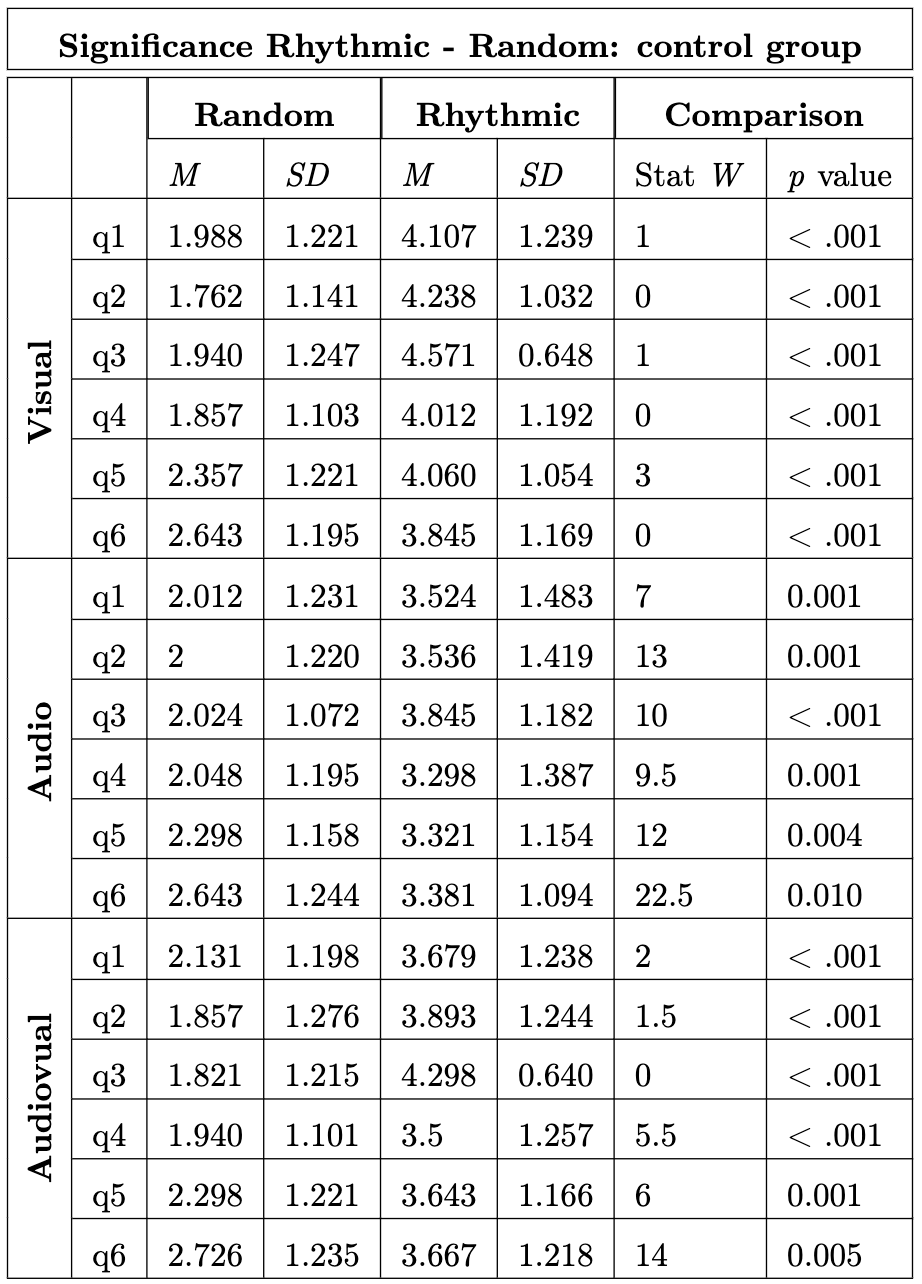
\includegraphics[width=\textwidth]{significance_tables/control_group.png}
        \caption{Statical values for rhythmic-random comparison: control group}
        \label{fig: significance rhythmic-random control} 
    \end{subfigure} 
    \begin{subfigure}[htbp]{0.33\textwidth}
        \centering
        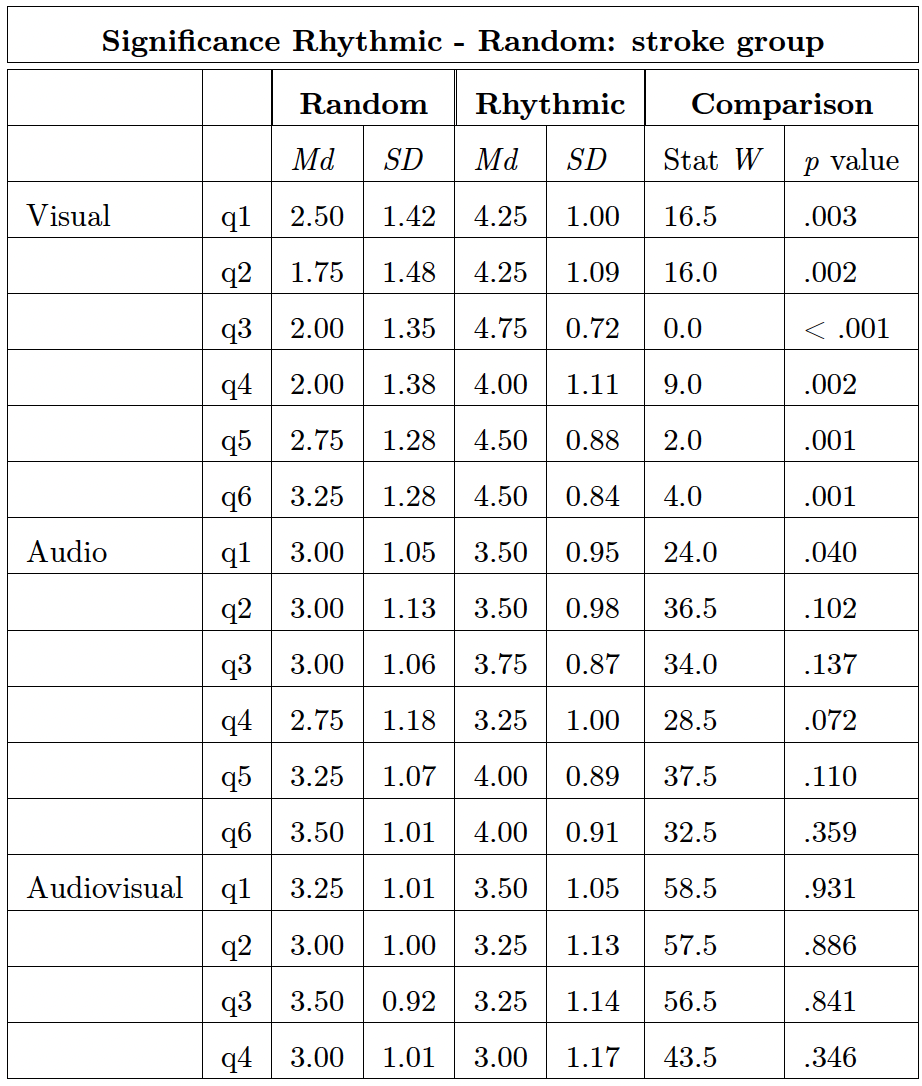
\includegraphics[width=\textwidth]{significance_tables/stroke_group.png}
        \caption{Statical values for rhythmic-random comparison: stroke group}
        \label{fig: significance rhythmic-random stroke} 
    \end{subfigure} 
    \caption{Statistical values for different conditions, comparing the two population groups}
    \label{fig: significance rhythmic-random}
\end{figure}

Furthermore, Figures \ref{fig: difference in population} represent the scores reported after each subjective question provided after the presentation of each sensory inputs in each experimental block, showing the differences between groups. From the statistical results reported in Table \ref{fig: significance pop} we can observe that patients with stroke provided higher scores in the random sequences compared to the healthy subjects group. In detail, such difference was detected in Q1 and Q2 corresponding to the visual input and in Q3 related to the audiovisual input. However, no differences between groups were detected for the rhythmic sequences (see Table \ref{fig: significance pop}).
\begin{figure}[htbp]
    \begin{subfigure}[htbp]{0.5\textwidth}
        \centering
        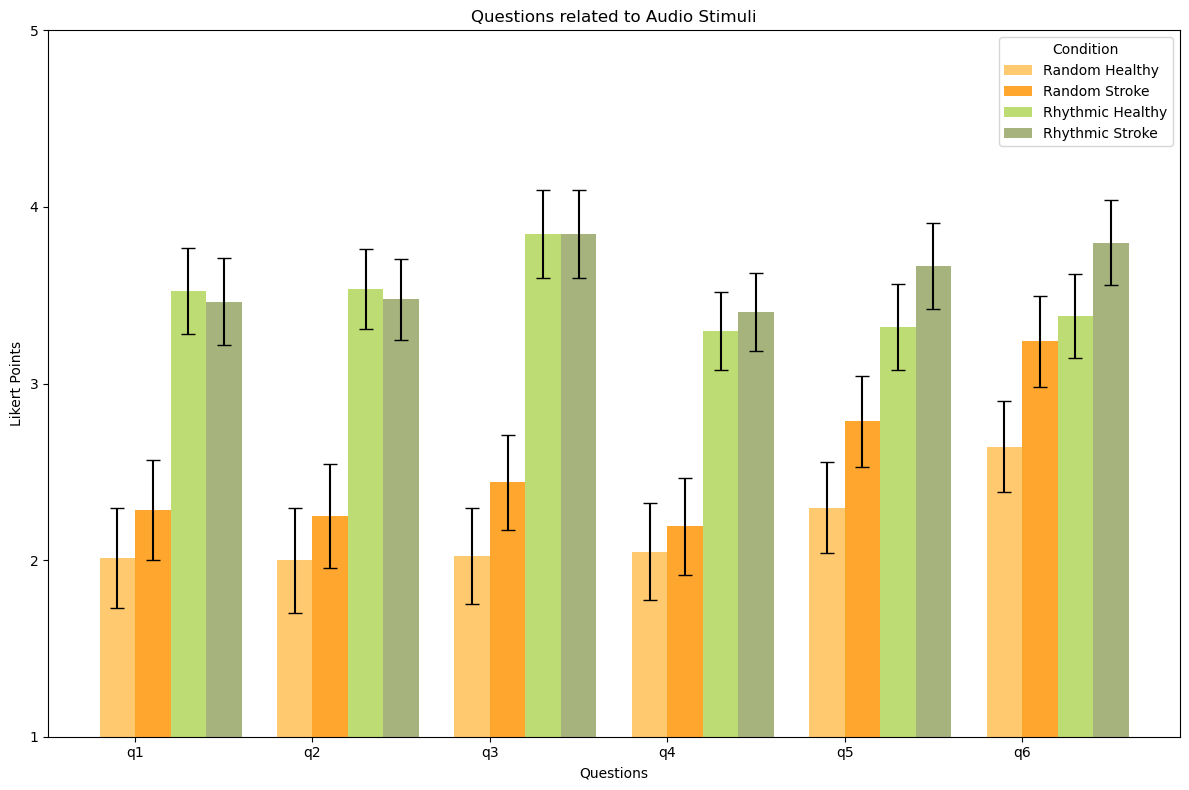
\includegraphics[width=\textwidth]{bar_plots/plot_pop_adio.png}
        \caption{Audio input: difference between population and condition}
        \label{fig: bar_visual_pop} 
    \end{subfigure} 
    \begin{subfigure}[htbp]{0.5\textwidth}
        \centering
        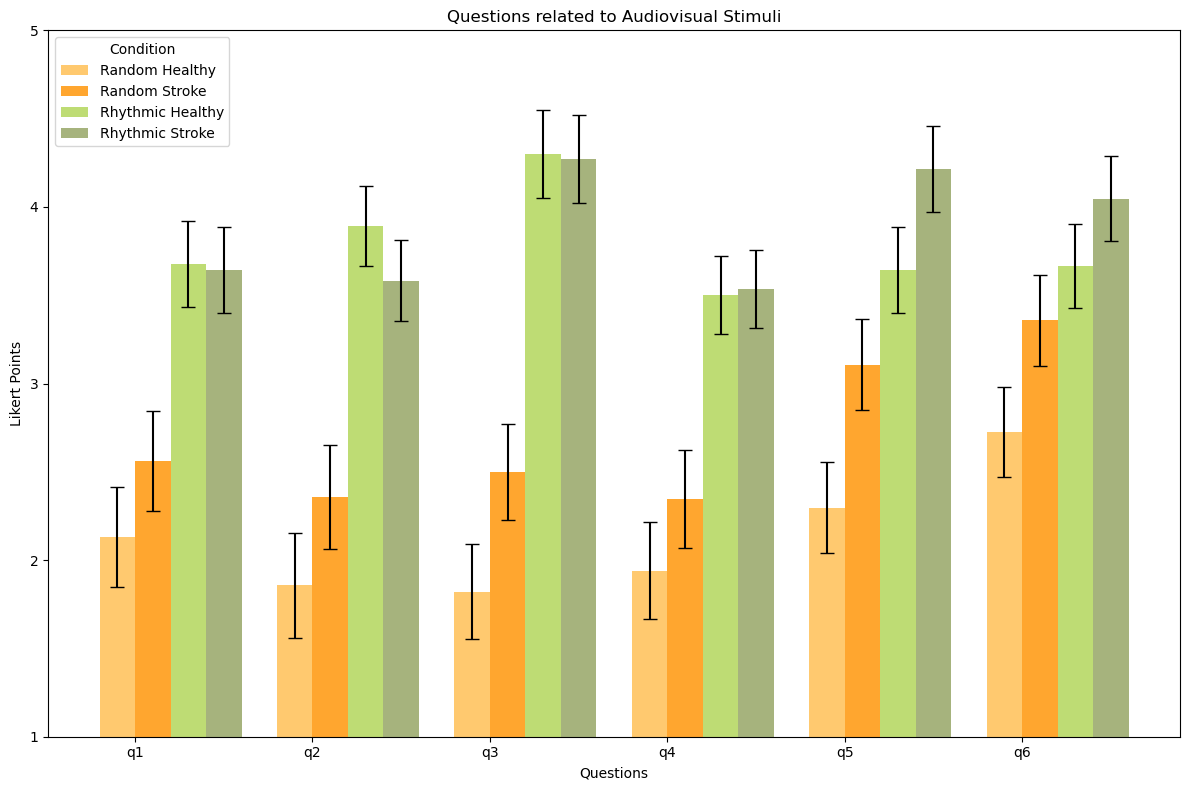
\includegraphics[width=\textwidth]{bar_plots/plot_pop_audiovisual.png}
        \caption{Audiovisual input: difference between population and condition}
        \label{fig: bar_audio_pop} 
    \end{subfigure} 
    \begin{subfigure}[htbp]{0.5\textwidth}
        \centering
        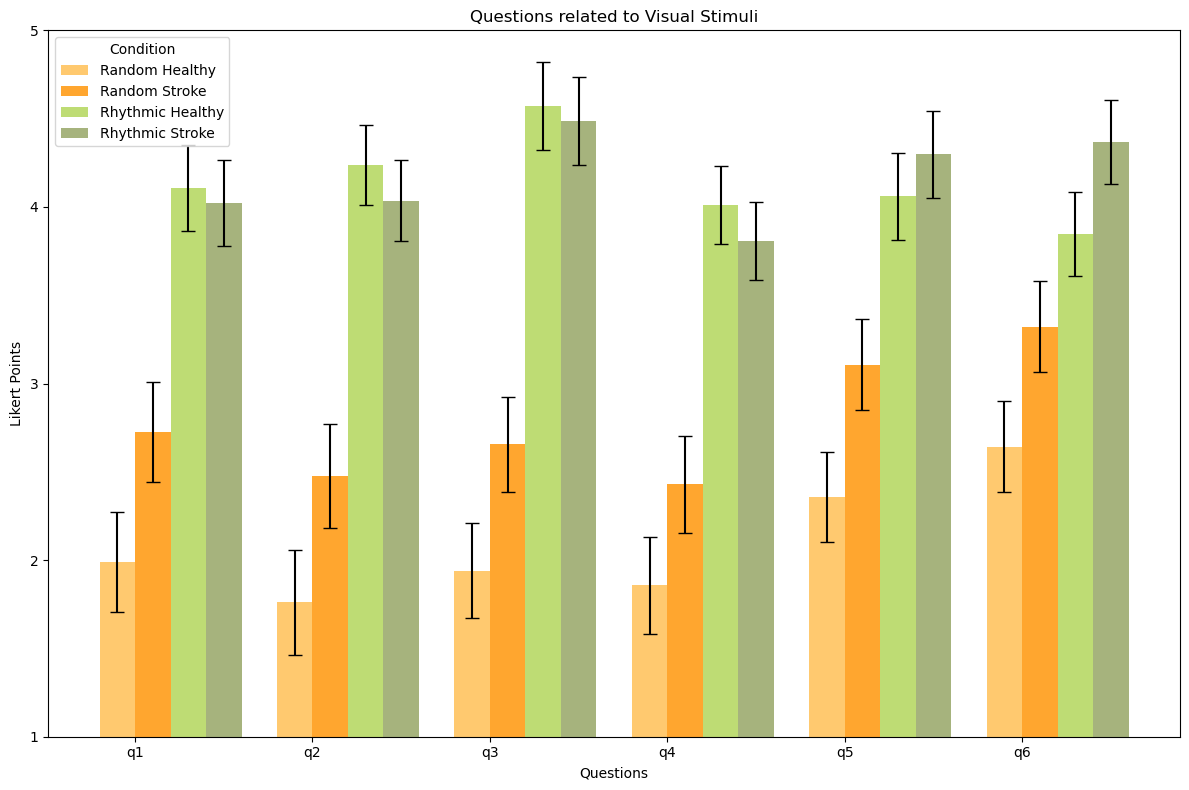
\includegraphics[width=\textwidth]{bar_plots/plot_pop_visual.png}
        \caption{Visual input: difference between population and condition}
        \label{fig: bar_audiovisual_pop} 
    \end{subfigure} 
    \caption{Bar plots representing difference between population and condition}
    \label{fig: difference in population}
\end{figure}
\begin{figure}[htbp]
    \centering
    \begin{subfigure}[htbp]{0.31\textwidth}
        \centering
        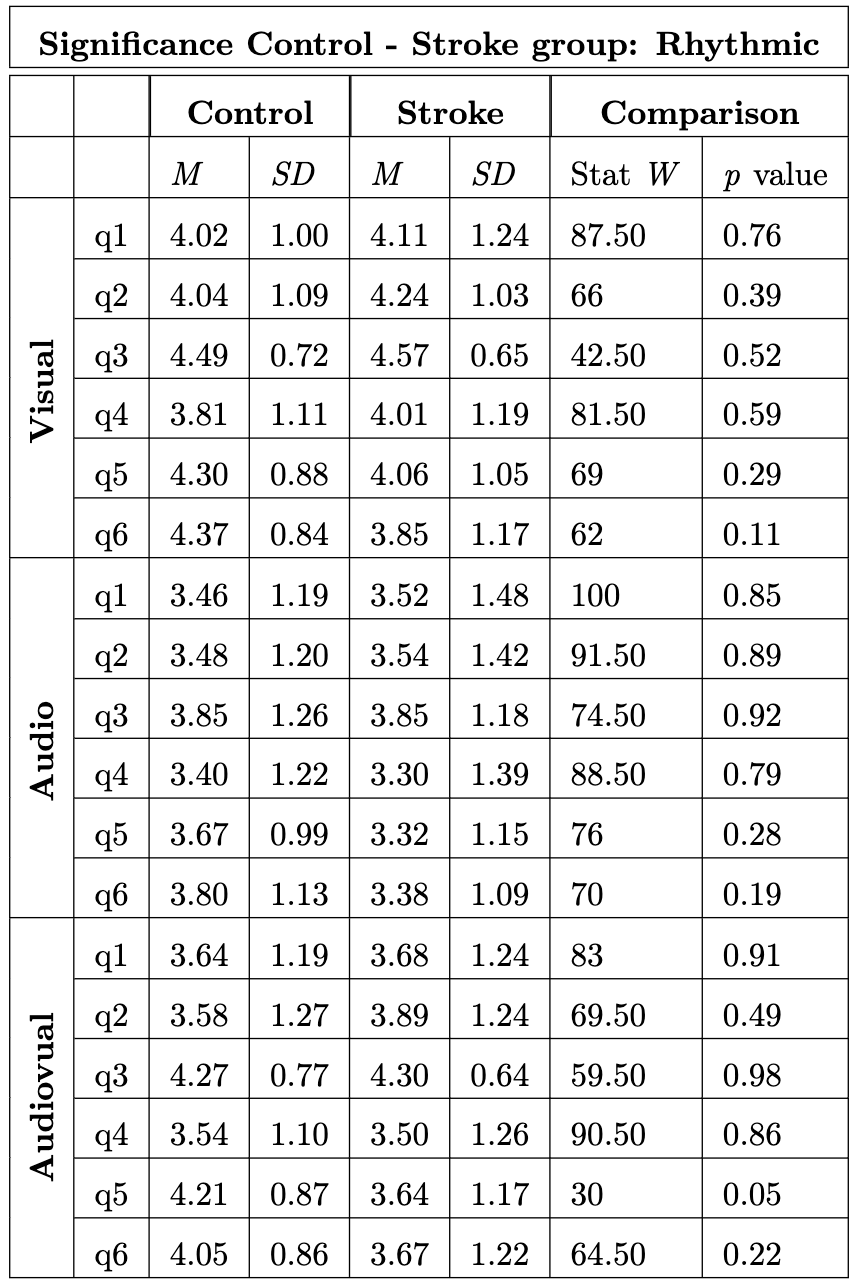
\includegraphics[width=\textwidth]{significance_tables/significance_control_pop.png}
        \caption{Statical values for rhythmic condition}
        \label{fig: significance_pop_rhythmic} 
    \end{subfigure} 
    \begin{subfigure}[htbp]{0.327\textwidth}
        \centering
        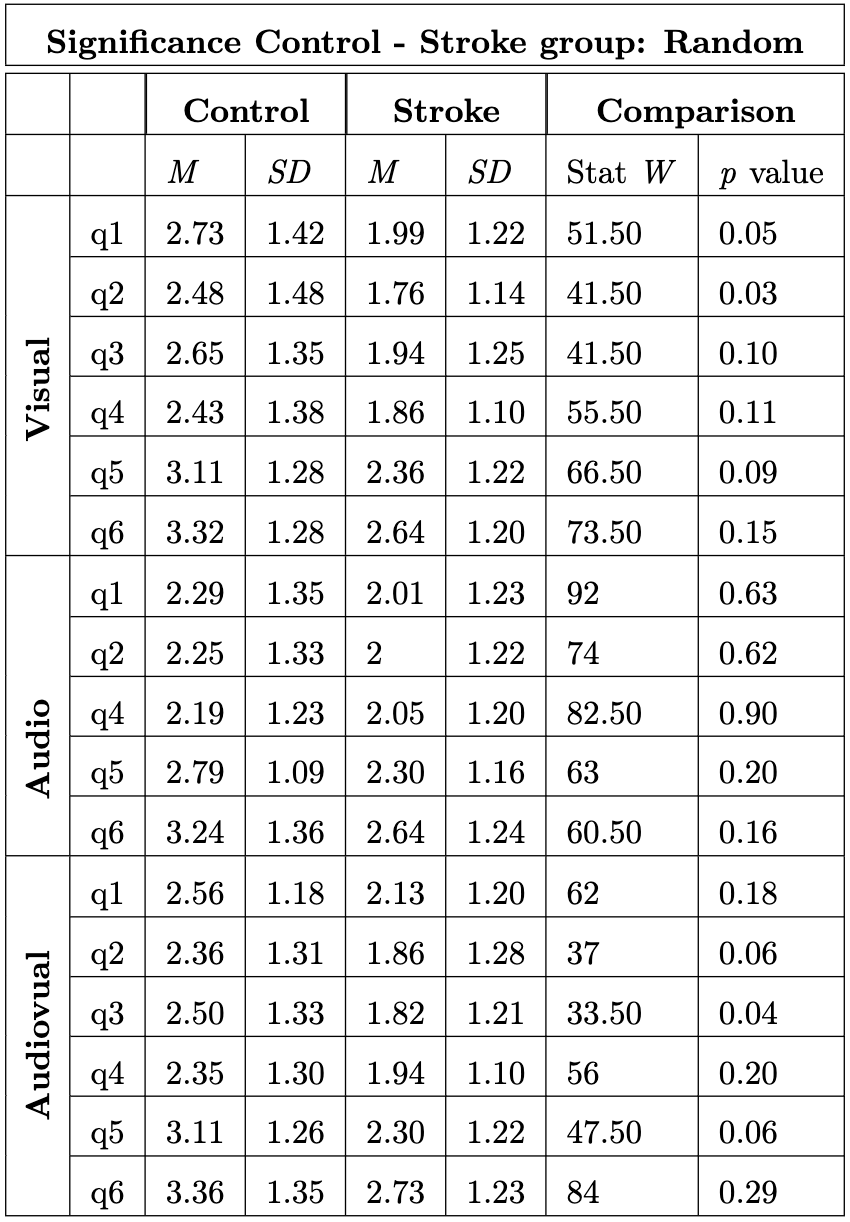
\includegraphics[width=\textwidth]{significance_tables/significance_random_pop.png}
        \caption{Statical values for random condition}
        \label{fig: significance_pop_random} 
    \end{subfigure} 
    \caption{Statistical values for different conditions, comparing the two population groups}
    \label{fig: significance pop}
\end{figure}

Moreover, we correlated the subjective report questions results obtained from Q2, after the observation of each sensory input presented in rhythmic sequences, with the mean power activity of the Occipital, Temporal and Sensorimotor ROIs, for each patient with stroke and healthy subjects group.\\
The results from the correlation show that there was no significant relationship between the mean power spectrum activity and the Q2 score in any of the three different ROIs (temporal, sensorimotor, occipital). However, in the patients with stroke group we observed a positive correlation between the mean power activity in the Temporal ROI and the scoring collected in Q2, in the auditory experimental block (Tables \ref{fig: correlation values q2: control} and \ref{fig correlation values q2: stroke}).
\begin{figure}[H]
    \centering
    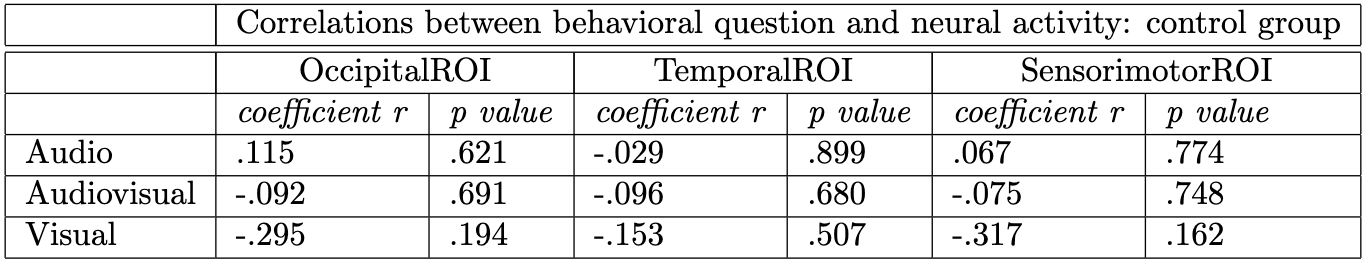
\includegraphics[width=0.75\textwidth]{scatter_plots/correlation_q2_control.png}
    \caption{Correlation values: Spearman correlation coefficient \textit{r} and \textit{p} value}
    \label{fig: correlation values q2: control} 
\end{figure}

\begin{figure}[H]
    \centering
    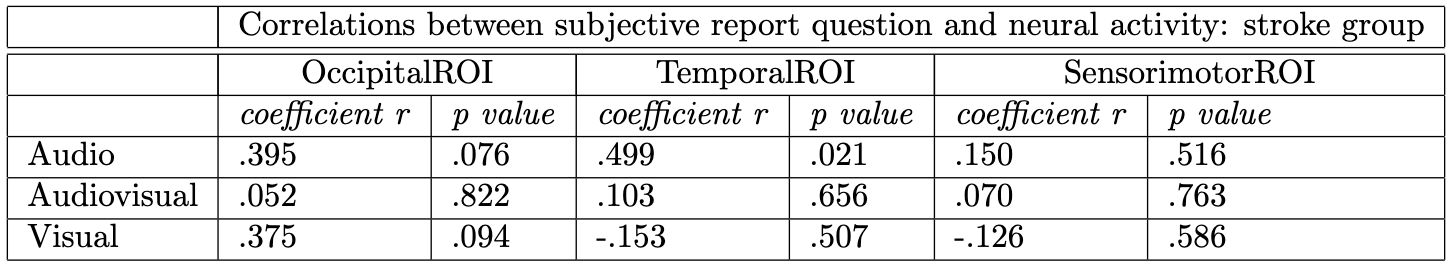
\includegraphics[width=0.75\textwidth]{scatter_plots/correlation_q2_stroke.png}
    \caption{Correlation values: Spearman correlation coefficient \textit{r} and \textit{p} value}
    \label{fig correlation values q2: stroke} 
\end{figure}

Finally, regarding the possible relationship between scoring collected in the Active-Q questionnaire (physical activity) and the mean average power in the sensorimotor ROI, the results did show any significant correlation in the healthy or patients with stroke group (Table \ref{fig: significance correlation activeq}). 
\begin{figure}[H]
    \centering
    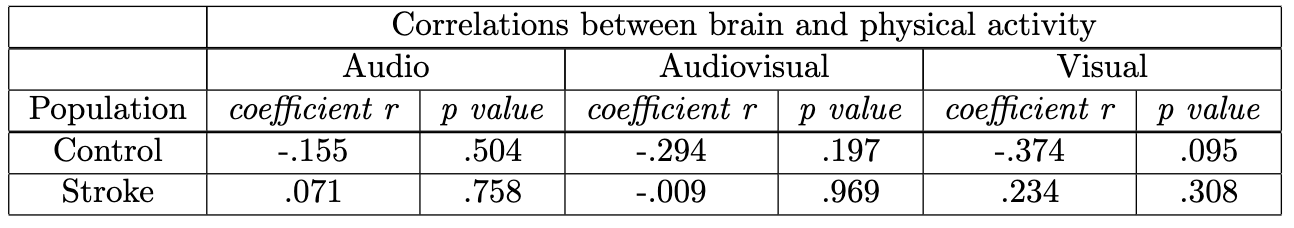
\includegraphics[width=0.75\textwidth]{significance_tables/correlation_activeq_.png}
    \caption{Correlation values: Spearman's correlation coefficient \textit{r} and \textit{p} value}
    \label{fig: significance correlation activeq} 
\end{figure}

%% previous part
% These results are better depicted by topographies representing the activity power spectrum only at the frequency of 2 Hz related to the three different stimuli, for both the rhythmic, random conditions and the difference between these two. Different graphs were built for each population group. \\
% In Figure \ref{fig: 3D topographies control group} we can analyze the neural activity of the control group: a strong activation of the temporal and sensorimotor areas were observed both in the audio and audiovisual rhythmic conditions, with a broader spread of the activity in the surrounding areas in the audio condition and the supplementary activation of the occipital lobe in the during the audiovisual stimuli. For what concerns the brain activation during the rhythmic visual stimuli, it can be seen clearly only in the occipital area. \\
% Moving to the topographies related to the random condition, the pattern of the brain activation appears as much weaker than the rhythmic condition, with a feeble arousal in some different brain regions. \\
% We can conclude that the frequency tagging effect is greater in the rhythmic conditions, with an activation of the ROIs that can be detected through the difference between the two conditions. 

% For what interests the stroke population, the encountered results (Figure \ref{fig: 3D topographies stroke group}) appear as slightly different from the control group. During the audio stimuli, the temporal and sensorimotor areas look activated, even if not as much as in the control group. Furthermore, strong lateralized arousal on the left side of the brain can be denoted in both the topographies related to the audio and audiovisual stimuli. On the other hand, the visual stimuli elicited a weaker activity in the stroke population compared to the control group, as well as a softer left sided activation than the audio and audiovisual ones. \\
% As in the control group, the random condition present a general weak brain activation, with the main difference of a noticeable arousal for what concerns the left side lateralization. \\
% Finally, the difference between the two conditions confirms the activation of the diverse ROIs related to the corresponding sensory inputs, resulting more feeble than the ones found in the control group. 

% For the analysis of the behavioral results, we firstly made distinct bar plots for each population group and sensory inputs. Firstly, in Figures \ref{fig: bar_visual_control}, \ref{fig: bar_audio_control} and \ref{fig: bar_audiovisual_control}, we can find the results related to the control group: here we can see that all the questions related to every sensory stimulus differ significantly between the random and rhythmic conditions, with higher values for the rhythmic condition. These results are confirmed by the report \textit{p} value in the statistical table in Figure \ref{fig: significance_control_pop}. \\
% From the graphical representation and the statistical results we can also detect that the question with the higher values in the rhythmic condition results to be the third one in all the stimuli, which refers to the perception of the movement fluidity by the subject. While this question appears as the one expressing the biggest difference between the two conditions, the last three questions in every sensory inputs (q4, q5 and q6) emerge to be the ones with lower differences between random and rhythmic, still being significant.
% \begin{figure}[htbp]
%     \begin{subfigure}[htbp]{0.5\textwidth}
%         \centering
%         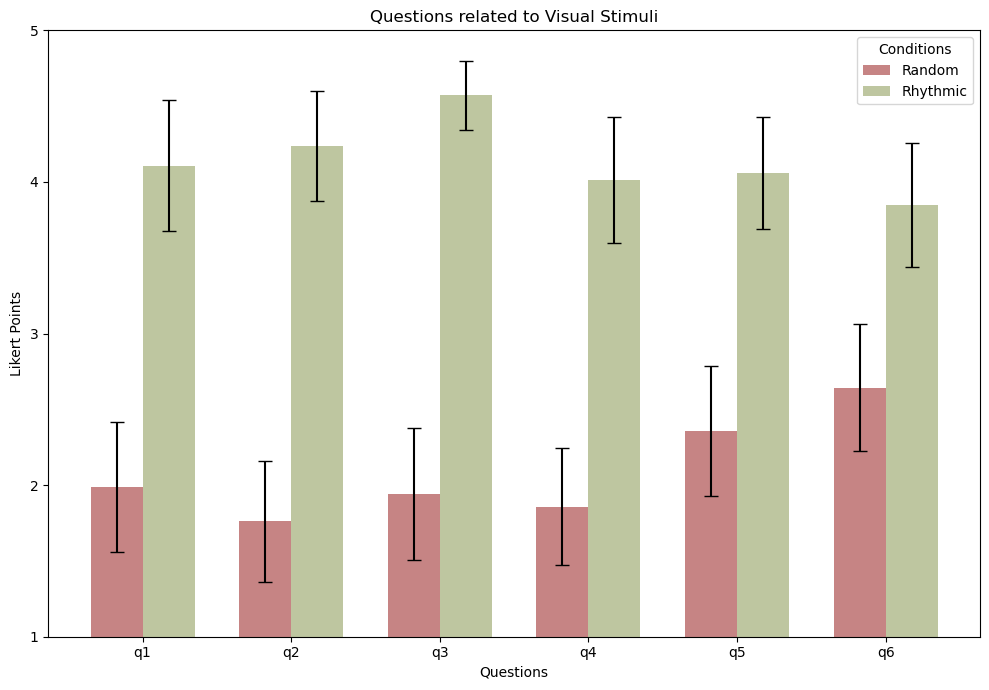
\includegraphics[width=\textwidth]{bar_plots/plotbar_visual_h.png}
%         \caption{Results of behavioral question in the visual condition in the control group}
%         \label{fig: bar_visual_control} 
%     \end{subfigure} 
%     \begin{subfigure}[htbp]{0.5\textwidth}
%         \centering
%         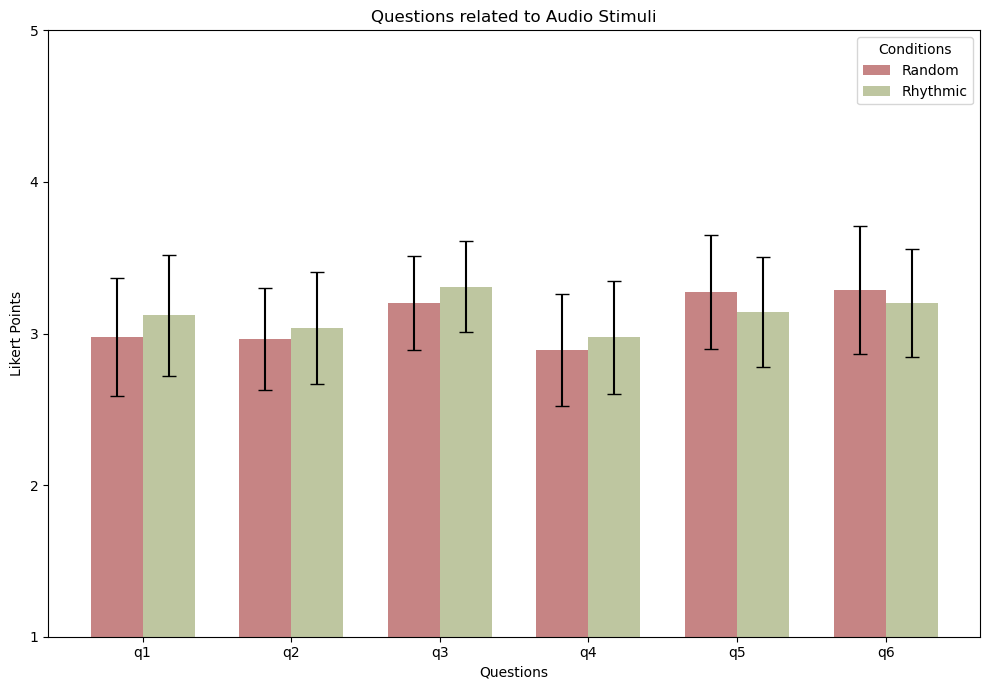
\includegraphics[width=\textwidth]{bar_plots/plotbar_audio_h.png}
%         \caption{Results of behavioral question in the audio condition in the control group}
%         \label{fig: bar_audio_control} 
%     \end{subfigure} 
%     \begin{subfigure}[htbp]{0.5\textwidth}
%         \centering
%         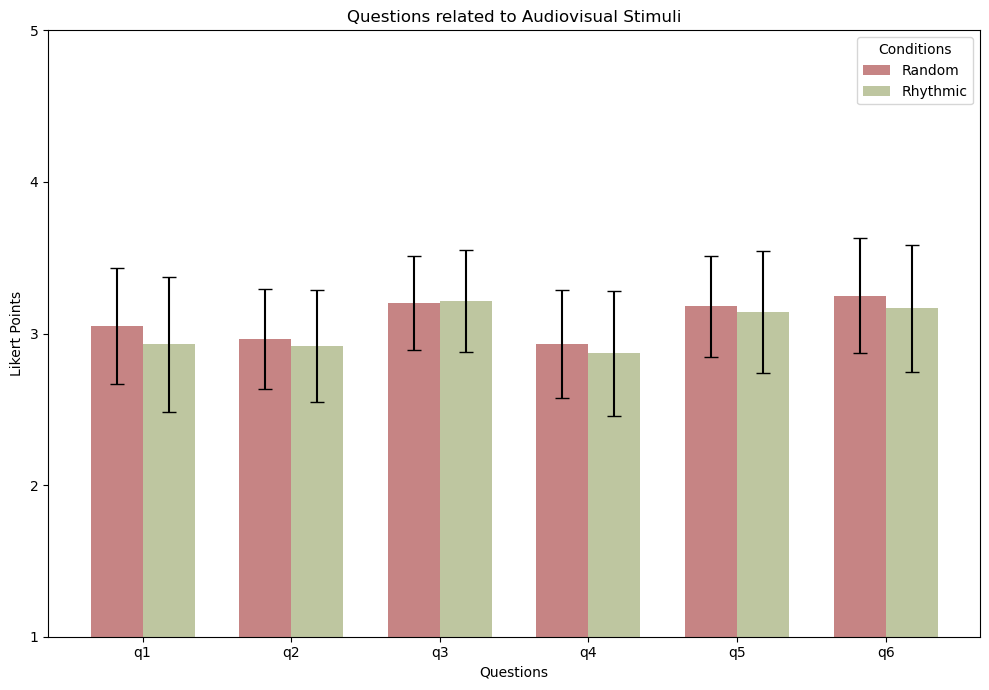
\includegraphics[width=\textwidth]{bar_plots/plotbar_audiovisual_h.png}
%         \caption{Results of behavioral question in the audiovisual condition in the control group}
%         \label{fig: bar_audiovisual_control} 
%     \end{subfigure} 
% \end{figure}

% Moving on to the outcome of the questions answered by the stroke group, which can be found in Figures: \ref{fig: bar_visual_stroke}, \ref{fig: bar_audio_stroke} and \ref{fig: bar_audiovisual_stroke}, similar results to the control group can be observed, with some minor differences. Firstly, we can affirm that equally to the previous results, a significant difference between all the questions related to the random and rhythmic for each sensory input, can be found (Figure \ref{fig: significance_stroke_pop}). \\ However, in the stroke population we can see that the difference appears to be generally lower compared to the one observed in the control group, except for question three in all the sensory inputs, question four in the audio stimulus and five in the audiovisual one. In general, we can conclude that the Likert values assigned to the questions referred to the random stimuli of all the sensory inputs appear as higher than in the control group.
% \begin{figure}[htbp]
%     \begin{subfigure}[b]{0.5\textwidth}
%         \centering
%         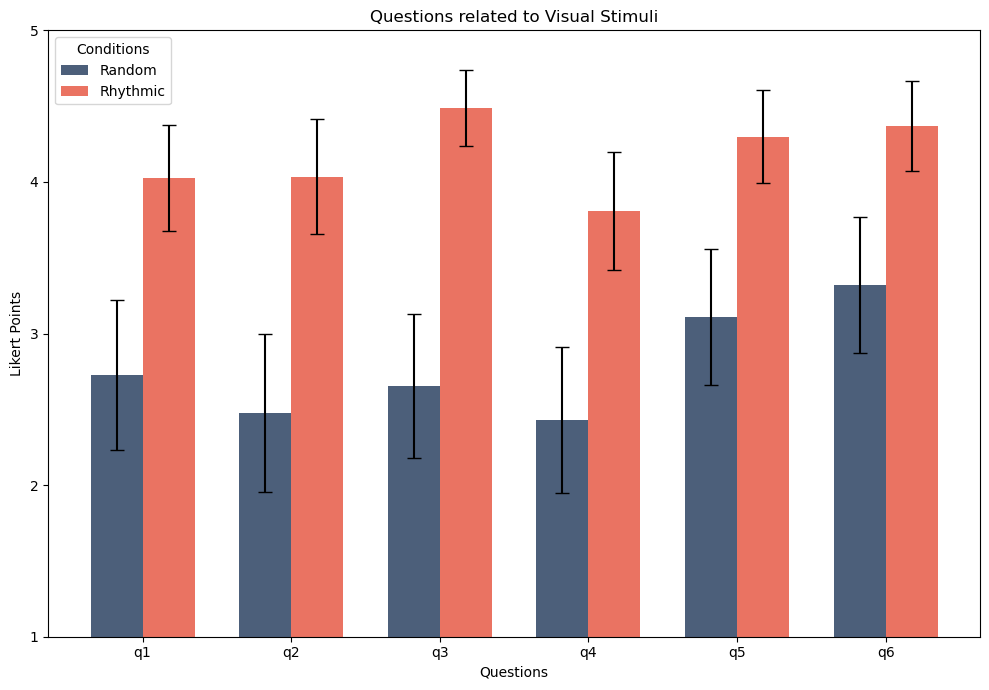
\includegraphics[width=\textwidth]{bar_plots/plotbar_visual_s.png}
%         \caption{Results of behavioral question in the visual condition in stroke population}
%         \label{fig: bar_visual_stroke} 
%     \end{subfigure} 
%     \begin{subfigure}[b]{0.5\textwidth}
%         \centering
%         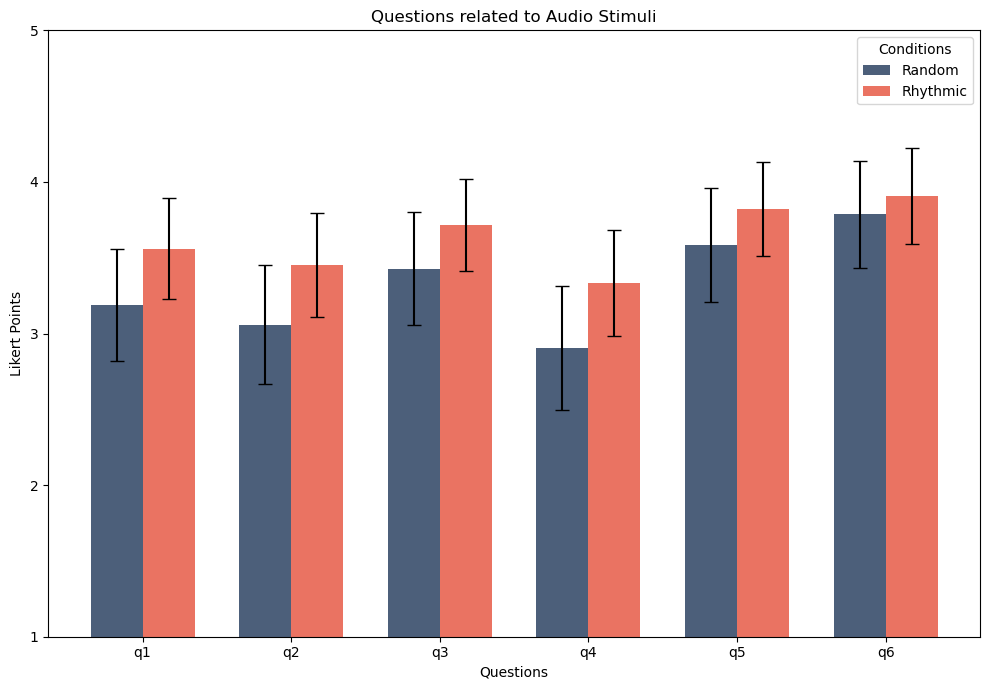
\includegraphics[width=\textwidth]{bar_plots/plotbar_audio_s.png}
%         \caption{Results of behavioral question in the audio condition in stroke population}
%         \label{fig: bar_audio_stroke} 
%     \end{subfigure} 
%     \begin{subfigure}[b]{0.5\textwidth}
%         \centering
%         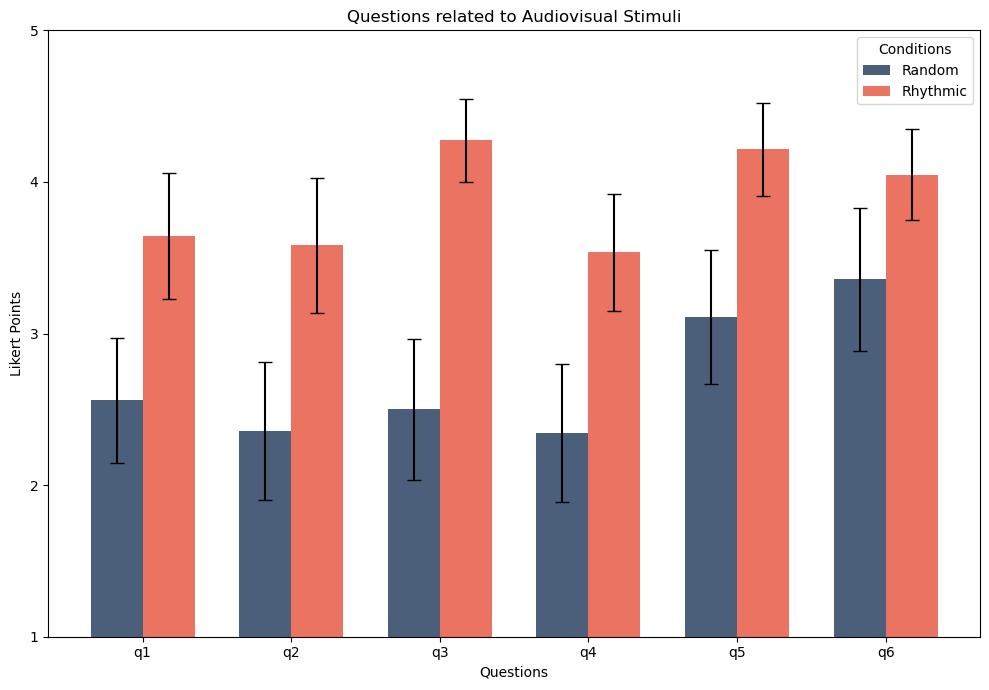
\includegraphics[width=\textwidth]{bar_plots/plotbar_audiovisual_s.png}
%         \caption{Results of behavioral question in the audiovisual condition in stroke population}
%         \label{fig: bar_audiovisual_stroke} 
%     \end{subfigure} 
% \end{figure}

% To confirm such difference between the two population groups, we decide to create a plot to visually compare them and to statistically measure their comparison. In Figure \ref{fig: mean_population_condition} we can recognize the distinction between the answers given by the stroke population and the control one to the random stimuli, and almost identical results for what concerns the rhythmic stimuli. If we then look at the statistical results (Figure \ref{fig: significance_total_mean_pop}) we can detect that the only significant result for the difference between the two population groups can be found for the answers related to the random visual inputs. 
% \begin{figure}[htbp]
%     \centering
%     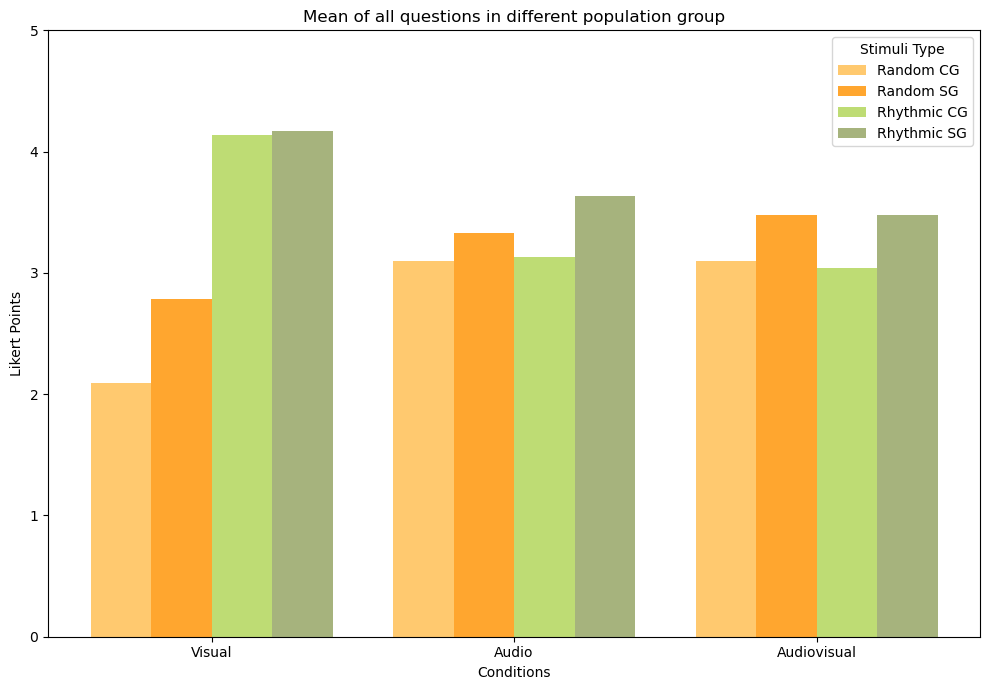
\includegraphics[width=0.5\textwidth]{bar_plots/mean stroke and control.png}
%     \caption{Mean of the results of all behavioral question divided by population groups (CG = control group; SG = stroke group)}
%     \label{fig: mean_population_condition} 
% \end{figure} 

% Later, we decided to correlate the most significant rhythmic \footnote{The choice of taking into account only the question in the rhythmic condition was made after seeing the results related to the difference between the two conditions: demonstrating that the rhythmic one got always higher values than the random.} question (q2) to the mean power activity of the Occipital, Temporal and Sensorimotor ROIs, dividing them always by population group. \\
% We can analyze the obtained results in Tables \ref{fig: correlation values q2: control} and \ref{fig: correlation values q2: stroke}. In the outcome for the control group we  observe that no correlation was found between the question related to the various sensory inputs and the power brain activity. Contrarily, looking at the results for the stroke population we can find a significant positive correlation between the values assigned to the behavioral question related to the audio stimuli and the neural activation in the Temporal ROI. Moving to the question related to the other sensory inputs (visual and audiovisual), no significant correlation with the mean power activity of the different ROIs could be found just as in the control group.

% Finally, we also aimed to understand if a possible correlation between the level of physical activity of the participants and their correspondent mean power activation in the Sensorimotor area could be present. The outcomes of our analysis showed no correlation between the level of physical activity and the activation of the sensorimotor area related to any of the sensory inputs (Table \ref{fig: significance correlation activeq}). 

% At beginning of our EEG data analysis we plotted the averaged signal-to-noise ratio (SNR) to observe if the desired brain signal would have been distinguishable from the background EEG activity. We can observe our plots of the rhythmic and random conditions of the two population groups in Figure \ref{fig: snr_rhythmic: control} and \ref{fig: snr_rhythmic: stroke} for the rhythmic condition; and in Figure \ref{fig: snr_random: control} and \ref{fig: snr_random: stroke} for the random one. \\
% The graphs don't seem to differ much between control and stroke groups. The rhythmic conditions, in which the frequency has been precisely set at 2 Hz, show the highest peak at 2 Hz and its harmonic (4 Hz), while a flat SNR values for what concerns the other frequency can be spotted. An exception regards the frequency of 1 Hz were the SNR appears still lower than the interested peaks, but higher than the other non target frequencies. On the other hand, in the SNR related to the random conditions it is possible to detect higher peaks at frequency of 1 Hz and its harmonics 2, 3 and 4 together with some lower noise in all the other frequencies. 

% We proceeded to calculate how the power spectrum representing the brain activity of our participant would change across our three regions of interest (occipital, temporal and sensorimotor) during the presentation of the different stimuli in the two conditions, expecting to find a peak amplitude at 2 Hz in the rhythmic condition, concordant with the previous results. We calculated separately for the two different population groups the grand average of the neural activity in the ROIs related to the different stimuli and the two separate conditions. \\
% Giving a general look to the plots of all the ROIs (which can be found starting from Figure \ref{fig: occipital ROI: control}) we can see a clear activation peak at 2 Hz in the rhythmic conditions and not in random ones for both of the population groups, as expected. However, it is also noticeable that the peaks found in all the ROIs power spectrum of the stroke group appear as lower than in the control group, denoting a weaker brain activation. \\
% For what concerns the stimuli in the random conditions the results appear to be almost the same in all the ROIs: the higher power activity can be observed at 1Hz and its harmonics even if with a lower value than the peaks at 2 Hz in the rhythmic conditions.

% Observing the plots for the specific ROIs, we can spot in the occipital ROI (Figures \ref{fig: occipital ROI: control} and \ref{fig: 3D topographies stroke group}) it is possible to spot the peak at 2 Hz clearly in the rhythmic condition of the visual and audiovisual sensory inputs, whilst in the temporal ROI (Figures \ref{fig: temporal ROI: control} and \ref{fig: temporal ROI: stroke}) it can mainly be observed it in the audio and audiovisual rhythmic conditions. Considering the last ROI, the sensorimotor area (Figures \ref{fig: sensorimotor ROI: control} and \ref{fig: sensorimotor ROI: stroke}), the activity peak at 2 Hz can only be noticed in the audio and audiovisual rhythmic conditions; in the visual one, a higher brain activity is spotted only in the control group at 1 Hz, similarly to its activity power spectrum in the temporal ROI.